\documentclass[11pt,oneside]{report}
\usepackage[utf8]{inputenc}
\usepackage[a4paper,top=2.4cm,bottom=2.4cm,left=2.5cm,right=2.5cm]{geometry}
\usepackage{graphicx}
\usepackage{xcolor}
\usepackage{amsmath,amssymb}
\usepackage{array,booktabs,tabularx,longtable}
\usepackage{float}
\usepackage{fancyvrb}
\usepackage{hyperref}

\definecolor{Navy}{HTML}{0B1F33}
\definecolor{Blue}{HTML}{16697A}
\definecolor{Cyan}{HTML}{2EC4B6}
\definecolor{Sky}{HTML}{4EA8DE}
\definecolor{Amber}{HTML}{F4A261}
\definecolor{Coral}{HTML}{E76F51}
\definecolor{Pale}{HTML}{EDF6F9}
\definecolor{SoftGray}{HTML}{F2F4F7}
\definecolor{MidGray}{HTML}{5C677D}

\hypersetup{
  colorlinks=true,
  linkcolor=Blue,
  citecolor=Blue,
  urlcolor=Blue,
  pdftitle={Proyecto Final Fase 1 - Diseño, Subneteo e Implementación Base en la Nube},
  pdfauthor={Grupo 1 - CC3067 Redes},
  pdfsubject={Propuesta técnica de red empresarial segmentada en AWS}
}

\setlength{\parindent}{0pt}
\setlength{\parskip}{0.65em}
\setlength{\emergencystretch}{2em}
\linespread{1.08}
\renewcommand{\arraystretch}{1.22}
\setcounter{secnumdepth}{3}
\setcounter{tocdepth}{2}
\renewcommand{\contentsname}{Contenido}
\renewcommand{\listfigurename}{Índice de figuras}
\renewcommand{\listtablename}{Índice de tablas}
\renewcommand{\chaptername}{Capítulo}
\renewcommand{\bibname}{Referencias}
\renewcommand{\figurename}{Figura}
\renewcommand{\tablename}{Tabla}
\renewcommand{\appendixname}{Anexo}

\newcolumntype{Y}{>{\raggedright\arraybackslash}X}
\newcolumntype{C}[1]{>{\centering\arraybackslash}p{#1}}
\newcolumntype{R}[1]{>{\raggedleft\arraybackslash}p{#1}}

\newcommand{\HRule}{\rule{\linewidth}{0.7pt}}
\newcommand{\code}[1]{\texttt{#1}}
\newcommand{\awsreserved}{\textcolor{Coral}{reservada por AWS}}
\newcommand{\statusok}{\textcolor{Blue}{\textbf{Verificado}}}

\newenvironment{infobox}[1][Nota técnica]
{\par\vspace{0.35em}\begin{center}\begin{minipage}{0.92\linewidth}\raggedright\textcolor{Blue}{\rule{\linewidth}{1.2pt}}\par\smallskip\textcolor{Blue}{\textbf{#1}}\par\smallskip}
{\smallskip\textcolor{Blue}{\rule{\linewidth}{1.2pt}}\end{minipage}\end{center}}

\newenvironment{warningbox}[1][Precaución]
{\begin{center}\begin{minipage}{0.92\linewidth}\textcolor{Coral}{\rule{\linewidth}{1.2pt}}\par\smallskip\textcolor{Coral}{\textbf{#1}}\par\smallskip}
{\smallskip\textcolor{Coral}{\rule{\linewidth}{1.2pt}}\end{minipage}\end{center}}

\makeatletter
\renewcommand\chapter{\if@openright\cleardoublepage\else\clearpage\fi
  \thispagestyle{plain}\global\@topnum\z@
  \@afterindentfalse\secdef\@chapter\@schapter}
\def\@makechapterhead#1{%
  \vspace*{8pt}%
  {\parindent\z@\raggedright\normalfont
    \textcolor{Cyan}{\Large\bfseries \chaptername\space\thechapter}\par\nobreak
    \vskip 8pt
    \textcolor{Navy}{\Huge\bfseries #1}\par\nobreak
    \vskip 10pt
    \textcolor{Cyan}{\rule{0.22\textwidth}{3pt}}\par\nobreak
    \vskip 24pt}}
\def\@makeschapterhead#1{%
  \vspace*{8pt}%
  {\parindent\z@\raggedright\normalfont
    \textcolor{Navy}{\Huge\bfseries #1}\par\nobreak
    \vskip 10pt
    \textcolor{Cyan}{\rule{0.22\textwidth}{3pt}}\par\nobreak
    \vskip 24pt}}
\makeatother

\graphicspath{{assets/diagrams/}{assets/generated/}{assets/screenshots/}{../../evidence/screenshots/}}


\begin{document}

\hypersetup{pageanchor=false}
\begin{titlepage}
  \thispagestyle{empty}
  \centering
  \textcolor{Blue}{\large Universidad del Valle de Guatemala}\\[2pt]
  \textcolor{MidGray}{Facultad de Ingeniería · Departamento de Ciencias de la Computación}\\[2pt]
  \textcolor{MidGray}{CC3067 Redes · Sección 10 · Grupo 1}

  \vspace{0.7cm}
  \HRule\\[0.45cm]
  {\Huge\bfseries\textcolor{Navy}{Proyecto Final: Fase 1}}\\[0.3cm]
  {\LARGE\bfseries\textcolor{Blue}{Diseño, Subneteo e Implementación Base en la Nube}}\\[0.22cm]
  {\large\textcolor{MidGray}{Propuesta técnica para RedNova GT}}
  \vspace{0.35cm}

  
\includegraphics[width=0.61\textwidth,height=10.4cm,keepaspectratio]{portada-red-nube.png}

  \vfill
  \begin{tabular}{@{}ll@{}}
    \textbf{Pablo Daniel Barillas Moreno} & 22193 \\
    \textbf{Andrés Rafael Chivalán} & 21534 \\
    \textbf{Roberto Emiliano Otoniel Camposeco Torres} & 23968 \\
  \end{tabular}

  \vspace{0.45cm}
  \textcolor{MidGray}{Guatemala, octubre de 2026}
\end{titlepage}

\hypersetup{pageanchor=true}
\pagenumbering{roman}
\pagestyle{plain}
\chapter*{Control del documento}
\addcontentsline{toc}{chapter}{Control del documento}

\begin{tabularx}{\textwidth}{>{\bfseries}p{4.1cm}Y}
Título & Proyecto Final: Fase 1 - Diseño, Subneteo e Implementación Base en la Nube \\
Organización propuesta & RedNova GT \\
Curso & CC3067 Redes, sección 10 \\
Equipo & Grupo 1 \\
Versión & 1.3 \\
Fecha objetivo & 19 de octubre de 2026 \\
Clasificación & Documento académico \\
Repositorio & \href{https://github.com/DanielBarillasM/Proyecto-final_Grupo-1_Redes_Sec-10.git}{\texttt{GitHub: Proyecto Final - Grupo 1}} \\
\end{tabularx}

\section*{Historial de revisión}

\begin{tabularx}{\textwidth}{C{1.65cm} C{2.4cm} Y Y}
\toprule
\textbf{Versión} & \textbf{Fecha} & \textbf{Descripción} & \textbf{Responsable} \\
\midrule
0.1 & 5/10/2026 & Definición de alcance, supuestos y arquitectura preliminar. & Grupo 1 \\
0.7 & 5/10/2026 & Incorporación de cálculos, diagramas, Terraform y controles de seguridad. & Grupo 1 \\
1.0 & 5/10/2026 & Compilación, validación técnica y revisión visual del entregable. & Grupo 1 \\
1.1 & 19/10/2026 & Ajustes editoriales solicitados, nueva captura PowerShell y auditoría final. & Grupo 1 \\
1.2 & 20/10/2026 & Evidencia de identidad y planificación en AWS, enlace al repositorio y actualización de pendientes. & Grupo 1 \\
1.3 & 20/10/2026 & Nota de ejecución final para controlar costos y actualización del riesgo de credenciales temporales. & Grupo 1 \\
\bottomrule
\end{tabularx}

\section*{Integrantes}

\begin{tabularx}{\textwidth}{Y C{3cm}}
\toprule
\textbf{Nombre} & \textbf{Carné} \\
\midrule
Pablo Daniel Barillas Moreno & 22193 \\
Andrés Rafael Chivalán & 21534 \\
Roberto Emiliano Otoniel Camposeco Torres & 23968 \\
\bottomrule
\end{tabularx}

\section*{Declaración de trazabilidad}

El informe distingue tres clases de afirmaciones: diseño propuesto, validación local reproducible y evidencia obtenida en servicios externos. Los resultados de herramientas se conservan en la carpeta \code{evidence/}; las credenciales, llaves privadas y estados de Terraform están excluidos del control de versiones. Las capturas añadidas acreditan autenticación y planificación contra AWS, pero no se presentan como evidencia de un \code{apply}, de recursos creados ni de conectividad entre instancias.

\tableofcontents
\listoffigures
\listoftables
\clearpage
\pagenumbering{arabic}
\pagestyle{headings}

\chapter{Resumen}

RedNova GT es una empresa guatemalteca ficticia que ofrece software de gestión comercial a pequeñas y medianas empresas. Su crecimiento exige separar lógicamente las funciones de Ventas, Tecnologías de la Información (TI), Data Center y acceso de visitantes. El presente documento propone trasladar ese ecosistema a Amazon Web Services (AWS), dentro de una nube privada virtual con direccionamiento IPv4 privado, controles de ruta y reglas de seguridad específicas.

La solución parte del bloque \code{10.10.0.0/24}. Mediante Variable Length Subnet Masking (VLSM) se reservan bloques diferentes según la demanda: \code{/26} para Visitas, \code{/26} para Ventas, \code{/27} para TI, \code{/28} para Data Center y \code{/28} para Administración. El último \code{/26} queda sin asignar para crecimiento. Esta distribución considera una particularidad esencial de AWS: en cada subred, las primeras cuatro direcciones y la última no pueden asignarse a recursos \cite{aws-subnet-sizing}. Por esa razón el cálculo operativo utiliza $2^{32-p}-5$ y no la fórmula tradicional $2^h-2$.

La arquitectura separa dos dominios de exposición. Visitas y Administración se asocian con una tabla de rutas pública; Ventas, TI y Data Center se asocian con una tabla privada que sólo conserva la ruta local de la VPC. Para la prueba de concepto, dos instancias pequeñas se ubican dentro de Ventas y reciben exclusivamente direcciones privadas. El acceso administrativo atraviesa un bastión temporal cuyo puerto SSH se limita a una sola dirección IPv4 \code{/32}. El tráfico ICMP entre las dos instancias se autoriza mediante un grupo de seguridad común.

La infraestructura se describe como código en Terraform y mantiene el cómputo deshabilitado de forma predeterminada para prevenir cargos involuntarios. El 22 de octubre de 2026 se ejecutó una ventana de prueba en \code{us-east-1}: Terraform creó 20 recursos, incluidas la VPC, cinco subredes, tres instancias EC2 y sus controles de red. Las instancias privadas de Ventas intercambiaron cuatro paquetes ICMP con 0\% de pérdida, mientras que el mismo intento desde el bastión obtuvo 100\% de pérdida. La carpeta \code{evidence/} conserva los registros y capturas correspondientes.

\begin{infobox}[Resultado principal]
El diseño satisface las capacidades solicitadas, utiliza bloques canónicos sin solapamiento y conserva 64 direcciones para crecimiento. La subred \code{10.10.0.64/26} asignada a Ventas ofrece 59 direcciones utilizables en AWS. El prototipo confirmó en la nube las direcciones privadas \code{10.10.0.71} y \code{10.10.0.79}, junto con la política de aislamiento prevista.
\end{infobox}

El repositorio reúne diagramas, scripts, Terraform, LaTeX y evidencia de AWS. Con el despliegue y las pruebas P-01 a P-05 documentadas, el alcance técnico de la Fase 1 queda completo.

\chapter{Contexto, alcance y supuestos}

\section{Contexto empresarial}

RedNova GT desarrolla una plataforma SaaS para inventario, facturación y análisis de ventas. El equipo de Ventas consulta demostraciones y oportunidades comerciales; TI administra sistemas, identidades y soporte; el Data Center aloja servicios internos y bases de datos; y los visitantes requieren conectividad aislada. Aunque la organización es ficticia, la separación responde a un patrón empresarial real: distintos grupos tienen necesidades y niveles de confianza distintos, por lo que compartir una red plana aumentaría tanto el dominio de falla como la superficie de exposición.

La fase no intenta construir una plataforma productiva de alta disponibilidad. Su propósito es producir un prototipo verificable que demuestre diseño, subneteo, configuración base y conectividad interna. La solución se concentra en una sola región y una sola zona de disponibilidad para reducir complejidad y costo. Una versión productiva debería duplicar los segmentos críticos en al menos dos zonas, incorporar monitoreo, registro centralizado, respaldo, balanceo y mecanismos administrados de acceso.

\section{Objetivos}

\subsection{Objetivo general}

Diseñar y prototipar en AWS una red empresarial segmentada para RedNova GT, demostrando mediante cálculos y pruebas que la asignación de direcciones, las rutas y los controles de acceso cumplen las necesidades declaradas.

\subsection{Objetivos específicos}

\begin{itemize}
  \item Comparar proveedores de nube con criterios técnicos, académicos y económicos.
  \item Traducir cantidades de usuarios y servidores a prefijos CIDR válidos para AWS.
  \item reservar espacio suficiente para crecimiento sin exceder el bloque principal.
  \item Separar segmentos públicos y privados mediante tablas de rutas explícitas.
  \item Aplicar mínimo privilegio con grupos de seguridad orientados a función.
  \item Automatizar la infraestructura para reducir errores manuales y permitir repetición.
  \item Demostrar conectividad ICMP entre dos instancias privadas dentro de Ventas.
  \item Documentar costos, riesgos, evidencias y el procedimiento de destrucción.
\end{itemize}

\section{Alcance incluido}

\begin{tabularx}{\textwidth}{p{4.4cm}Y}
\toprule
\textbf{Componente} & \textbf{Cobertura de esta fase} \\
\midrule
Direccionamiento & Una VPC IPv4 privada, cinco subredes implementables y un bloque de reserva. \\
Enrutamiento & Tabla pública con ruta por Internet Gateway y tabla privada sin salida directa. \\
Seguridad & Dos grupos de seguridad, restricción SSH por \code{/32} e ICMP interno controlado. \\
Cómputo & Un bastión temporal y dos instancias pequeñas de prueba cuando se habilita \code{enable\_compute}. \\
Automatización & Código Terraform, variables, salidas, etiquetas y scripts de validación. \\
Pruebas & Capacidad CIDR, no solapamiento, validación Terraform y ping mediante direcciones privadas. \\
Documentación & Informe, diagramas, evidencias y README de la fase. \\
\bottomrule
\end{tabularx}

\section{Fuera de alcance}

Quedan fuera de esta fase: arquitectura multirregión, alta disponibilidad en múltiples zonas, VPN hacia oficinas físicas, directorio corporativo, balanceadores, bases de datos administradas, inspección profunda de paquetes, IPv6, observabilidad completa, pruebas de rendimiento y recuperación ante desastres. Estos elementos aparecen como recomendaciones de evolución, no como componentes supuestamente implementados.

\section{Supuestos y restricciones}

\begin{longtable}{p{4.0cm}p{8.2cm}p{2.1cm}}
\toprule
\textbf{Supuesto} & \textbf{Justificación e impacto} & \textbf{Estado} \\
\midrule
\endfirsthead
\toprule
\textbf{Supuesto} & \textbf{Justificación e impacto} & \textbf{Estado} \\
\midrule
\endhead
30 visitantes concurrentes & El enunciado no cuantifica Visitas. Se adopta una carga razonable que exige \code{/26} en AWS y deja margen. & Explícito \\
25 dispositivos en Ventas & Se interpreta una dirección primaria por colaborador, más crecimiento operativo separado. & Dado \\
15 dispositivos en TI & Se interpreta una dirección primaria por colaborador; \code{/27} deja doce libres. & Dado \\
5 servidores lógicos & La cifra dimensiona Data Center; no obliga a ejecutar cinco EC2 durante el prototipo. & Dado \\
Una zona de disponibilidad & Es suficiente para demostrar segmentación, pero no ofrece tolerancia a la falla de zona. & Limitación \\
Acceso administrativo conocido & El equipo debe conocer su IPv4 pública y expresarla como \code{/32}. & Operativo \\
Cuenta con permisos mínimos & Se requieren permisos para VPC, EC2, grupos de seguridad, llaves y etiquetas. & Externo \\
\bottomrule
\end{longtable}

\begin{warningbox}[Restricción económica]
El diseño evita NAT Gateway y direcciones públicas innecesarias. Sin embargo, AWS cobra por direcciones IPv4 públicas asociadas y ociosas \cite{aws-vpc-pricing}. El bastión sólo debe existir durante la prueba y su dirección debe liberarse al destruir el prototipo.
\end{warningbox}

\chapter{Selección y justificación del proveedor}

\section{Método de evaluación}

La decisión se tomó con una matriz multicriterio. Cada proveedor recibe una puntuación de 1 a 5, donde 1 indica ajuste bajo y 5 ajuste excelente. La nota ponderada se calcula como:

\[
S_j = \sum_{i=1}^{n} w_i r_{ij}, \qquad \sum_{i=1}^{n}w_i=1
\]

Aquí, $S_j$ es el resultado del proveedor $j$, $w_i$ el peso del criterio $i$ y $r_{ij}$ su calificación. Los pesos priorizan la adecuación de red y el beneficio académico porque el objetivo de la fase es aprender segmentación y demostrarla con bajo riesgo económico.

\begin{table}[H]
\centering
\caption{Criterios utilizados para seleccionar la nube}
\begin{tabularx}{\textwidth}{Y C{2.1cm} Y}
\toprule
\textbf{Criterio} & \textbf{Peso} & \textbf{Interpretación} \\
\midrule
Ajuste de red & 30\% & Claridad del modelo VPC, subredes, rutas y reglas de seguridad. \\
Beneficio académico & 25\% & Facilidad de construir una prueba corta con créditos o capa aplicable a la cuenta. \\
Documentación & 20\% & Cobertura oficial, ejemplos y capacidad de citar comportamiento exacto. \\
Infraestructura como código & 15\% & Madurez del proveedor Terraform y reproducibilidad. \\
Control de costo & 10\% & Visibilidad, etiquetas, presupuestos y facilidad de desmantelamiento. \\
\bottomrule
\end{tabularx}
\end{table}

\begin{figure}[H]
\centering
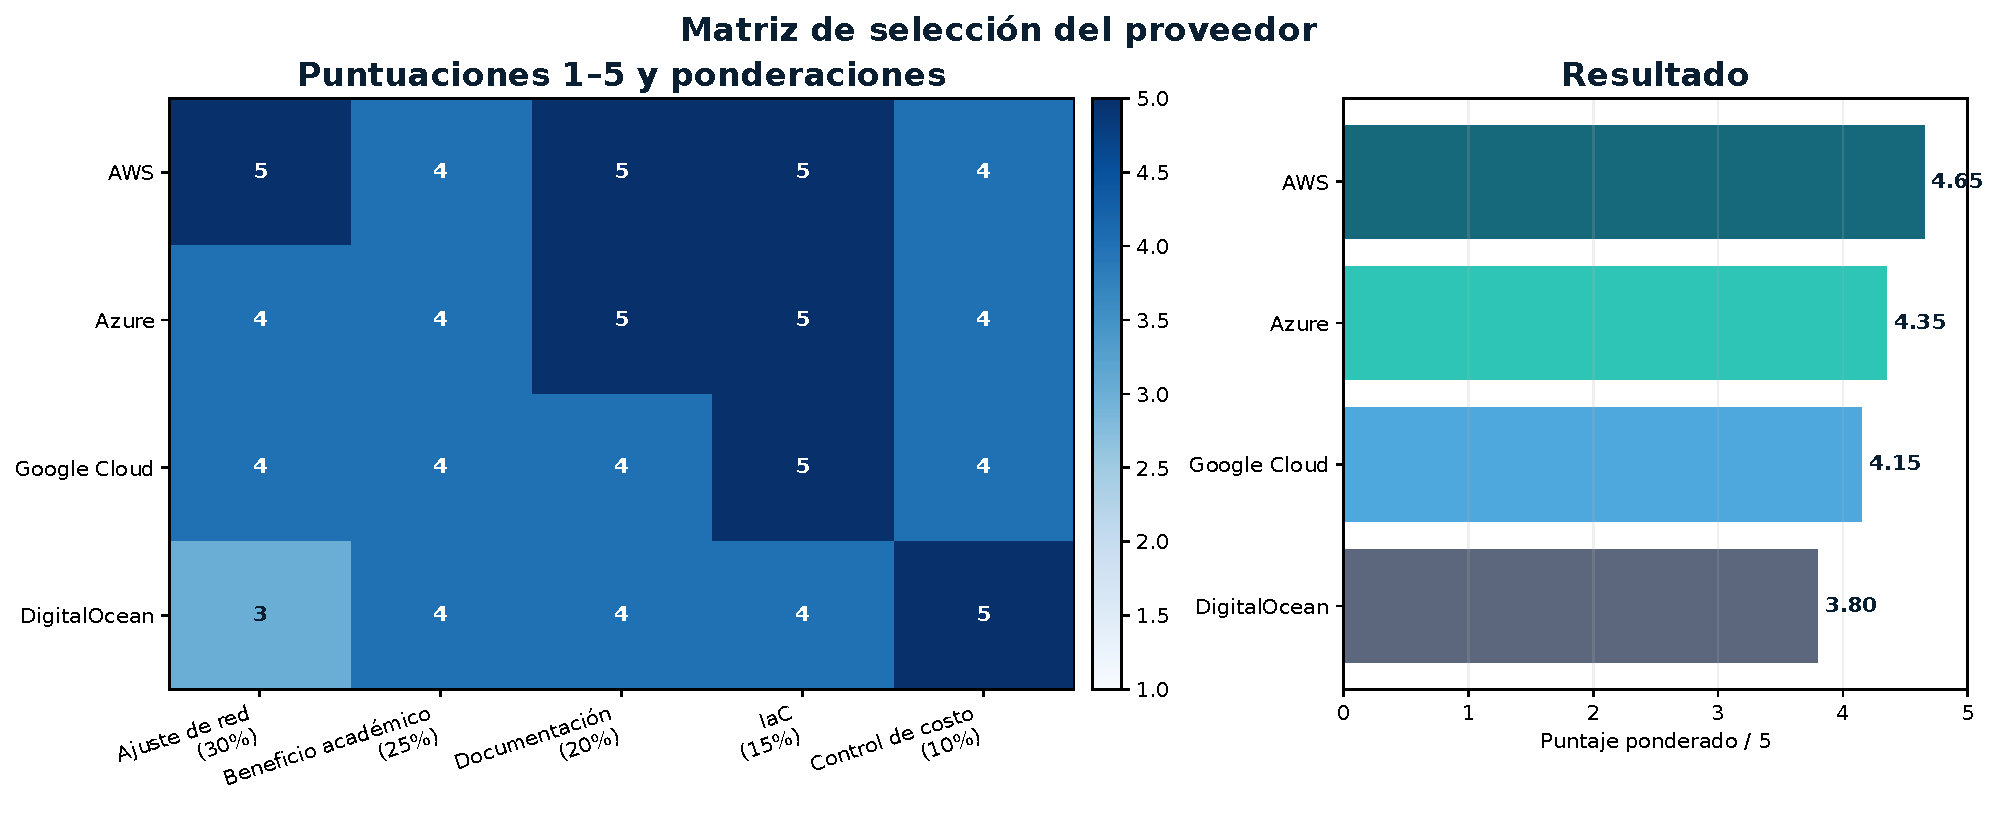
\includegraphics[width=\textwidth]{matriz-proveedores.pdf}
\caption{Matriz ponderada de selección del proveedor. Elaboración propia.}
\label{fig:providers}
\end{figure}

\section{Interpretación del resultado}

AWS obtiene 4.65/5, seguido por Azure con 4.35, Google Cloud con 4.15 y DigitalOcean con 3.80. La diferencia no implica que AWS sea universalmente superior; significa que ofrece el mejor ajuste para este prototipo y para los criterios definidos. Su documentación distingue con precisión subredes públicas y privadas: una subred es pública cuando su tabla contiene una ruta hacia un Internet Gateway, mientras una subred sin dicha ruta es privada \cite{aws-internet-gateway}.

Azure y Google Cloud ofrecen capacidades equivalentes y proveedores Terraform maduros, pero la nomenclatura de Amazon VPC se alinea de forma directa con los objetivos docentes del enunciado. DigitalOcean reduce complejidad operativa, pero esa misma simplificación ofrece menos elementos para demostrar rutas y controles de seguridad con el nivel de detalle buscado.

\section{Justificación técnica de AWS}

\subsection{Correspondencia entre conceptos académicos y recursos}

\begin{tabularx}{\textwidth}{p{4.2cm}Y}
\toprule
\textbf{Concepto de redes} & \textbf{Representación en el prototipo} \\
\midrule
Red empresarial privada & Amazon VPC con bloque RFC 1918 \code{10.10.0.0/24}. \\
Segmentación lógica & Cinco recursos \code{aws\_subnet} con CIDR no superpuestos. \\
Gateway & Internet Gateway adjunto a la VPC. \\
Enrutamiento & Tablas pública y privada asociadas explícitamente con las subredes. \\
Filtrado con estado & Grupos de seguridad para bastión y Ventas. \\
Host de prueba & Instancias EC2 con interfaces dentro de Ventas. \\
Documentación reproducible & Recursos declarativos y salidas de Terraform. \\
\bottomrule
\end{tabularx}

\subsection{Trazabilidad y automatización}

Terraform transforma la arquitectura en recursos declarativos revisables. El archivo de configuración permite detectar cambios, estandarizar etiquetas y recrear el entorno sin repetir pasos de consola. HashiCorp distribuye Terraform como un ejecutable multiplataforma y documenta el flujo de inicialización, planificación y aplicación \cite{terraform-install}. En el repositorio, cada componente se separa por propósito: proveedor, variables, red, seguridad, cómputo y salidas.

\subsection{Control del costo}

La elección se acompaña de límites concretos: el cómputo no se crea por defecto; no se incorpora NAT Gateway; sólo el bastión recibe una dirección pública; todas las instancias usan volúmenes pequeños y cifrados; y los recursos llevan la etiqueta \code{DeleteAfter=2026-10-19}. AWS recomienda rastrear recursos durante su ciclo de vida y retirar los elementos de prueba cuando dejan de ser necesarios \cite{aws-track-resources}. La automatización facilita cumplir esa práctica con \code{terraform destroy}.

\section{Decisión}

Se selecciona AWS para la Fase 1. La decisión está condicionada al alcance académico y debe reevaluarse si el proyecto evoluciona a producción, cambia el perfil de costos, requiere residencia de datos específica o necesita servicios administrados que alteren la comparación.

\chapter{Análisis de requerimientos}

\section{Requerimientos funcionales}

\begin{longtable}{C{1.2cm}p{5.0cm}p{7.3cm}}
\toprule
\textbf{ID} & \textbf{Requerimiento} & \textbf{Criterio de aceptación} \\
\midrule
\endfirsthead
\toprule
\textbf{ID} & \textbf{Requerimiento} & \textbf{Criterio de aceptación} \\
\midrule
\endhead
RF-01 & Crear una red empresarial en la nube. & Existe una VPC con CIDR \code{10.10.0.0/24} y DNS habilitado. \\
RF-02 & Segmentar Ventas. & La subred soporta al menos 25 direcciones asignables a recursos. \\
RF-03 & Segmentar TI. & La subred soporta al menos 15 direcciones asignables a recursos. \\
RF-04 & Segmentar Data Center. & La subred soporta al menos cinco servidores. \\
RF-05 & Segmentar Visitas. & Existe un bloque separado, con capacidad documentada para 30 conexiones concurrentes. \\
RF-06 & Demostrar conectividad. & Cuatro respuestas exitosas de ICMP entre dos IP privadas de Ventas. \\
RF-07 & Conservar configuración. & Terraform describe todos los recursos base y valida sin errores. \\
RF-08 & Documentar implementación. & Cada etapa indica entrada, acción, verificación y evidencia esperada. \\
\bottomrule
\end{longtable}

\section{Requerimientos no funcionales}

\begin{itemize}
  \item \textbf{Seguridad:} acceso denegado por defecto entre dominios; SSH limitado a una IP administrativa; metadatos EC2 únicamente mediante IMDSv2; volúmenes cifrados.
  \item \textbf{Reproducibilidad:} una segunda ejecución con las mismas variables debe producir una arquitectura equivalente.
  \item \textbf{Auditabilidad:} nombres, etiquetas, salidas y archivos de evidencia deben permitir relacionar la documentación con el despliegue.
  \item \textbf{Economía:} evitar componentes permanentes y eliminar recursos al terminar la prueba.
  \item \textbf{Legibilidad:} diagramas vectoriales, tablas autoexplicativas y referencias cruzadas.
  \item \textbf{Mantenibilidad:} separación modular entre red, seguridad y cómputo.
\end{itemize}

\section{Criterios de aceptación y evidencia}

\begin{table}[H]
\centering
\caption{Trazabilidad entre entregables y evidencia}
\begin{tabularx}{\textwidth}{p{4.3cm}Y p{3.2cm}}
\toprule
\textbf{Entregable solicitado} & \textbf{Respuesta del proyecto} & \textbf{Evidencia} \\
\midrule
Justificación del proveedor & Capítulo 3 y matriz ponderada. & Figura \ref{fig:providers} \\
Diagrama de red & Arquitectura pública/privada y flujo administrativo. & Figura \ref{fig:architecture} \\
Cálculos de segmentación & Derivación matemática, tabla detallada y mapa VLSM. & Capítulo 6 \\
Pasos de implementación & Flujo Terraform y descripción recurso por recurso. & Capítulo 8 \\
Prueba de ping & Procedimiento, comando, salida y criterios de éxito. & Capítulo 9 \\
Archivos de configuración & Módulos Terraform y scripts versionados. & Anexos y repositorio \\
Control de costos & Diseño temporal, etiquetas y destrucción. & Capítulo 11 \\
\bottomrule
\end{tabularx}
\end{table}

\section{Riesgos de interpretación}

La palabra ``privada'' puede describir tanto un bloque de direcciones internas como una subred sin ruta directa a Internet. Para evitar ambigüedad, este documento aplica la definición operativa de AWS: Ventas, TI y Data Center no tienen ruta \code{0.0.0.0/0} hacia un Internet Gateway. Visitas y Administración sí se asocian con una tabla pública, pero el acceso real depende además de una dirección pública y de reglas explícitas. Una ruta, por sí sola, no abre puertos.

\chapter{Diseño de la red}

\section{Vista general}

La solución utiliza una VPC no predeterminada para que cada ruta y asociación sea deliberada. El bloque \code{10.10.0.0/24} pertenece al espacio privado de RFC 1918 y contiene 256 direcciones. Cinco bloques se materializan como subredes; el sexto se conserva como reserva lógica. Todas las subredes del prototipo se colocan en la primera zona disponible de la región elegida. AWS establece que cada subred pertenece por completo a una zona de disponibilidad y no puede abarcar varias \cite{aws-configure-subnets}.

\begin{figure}[H]
\centering
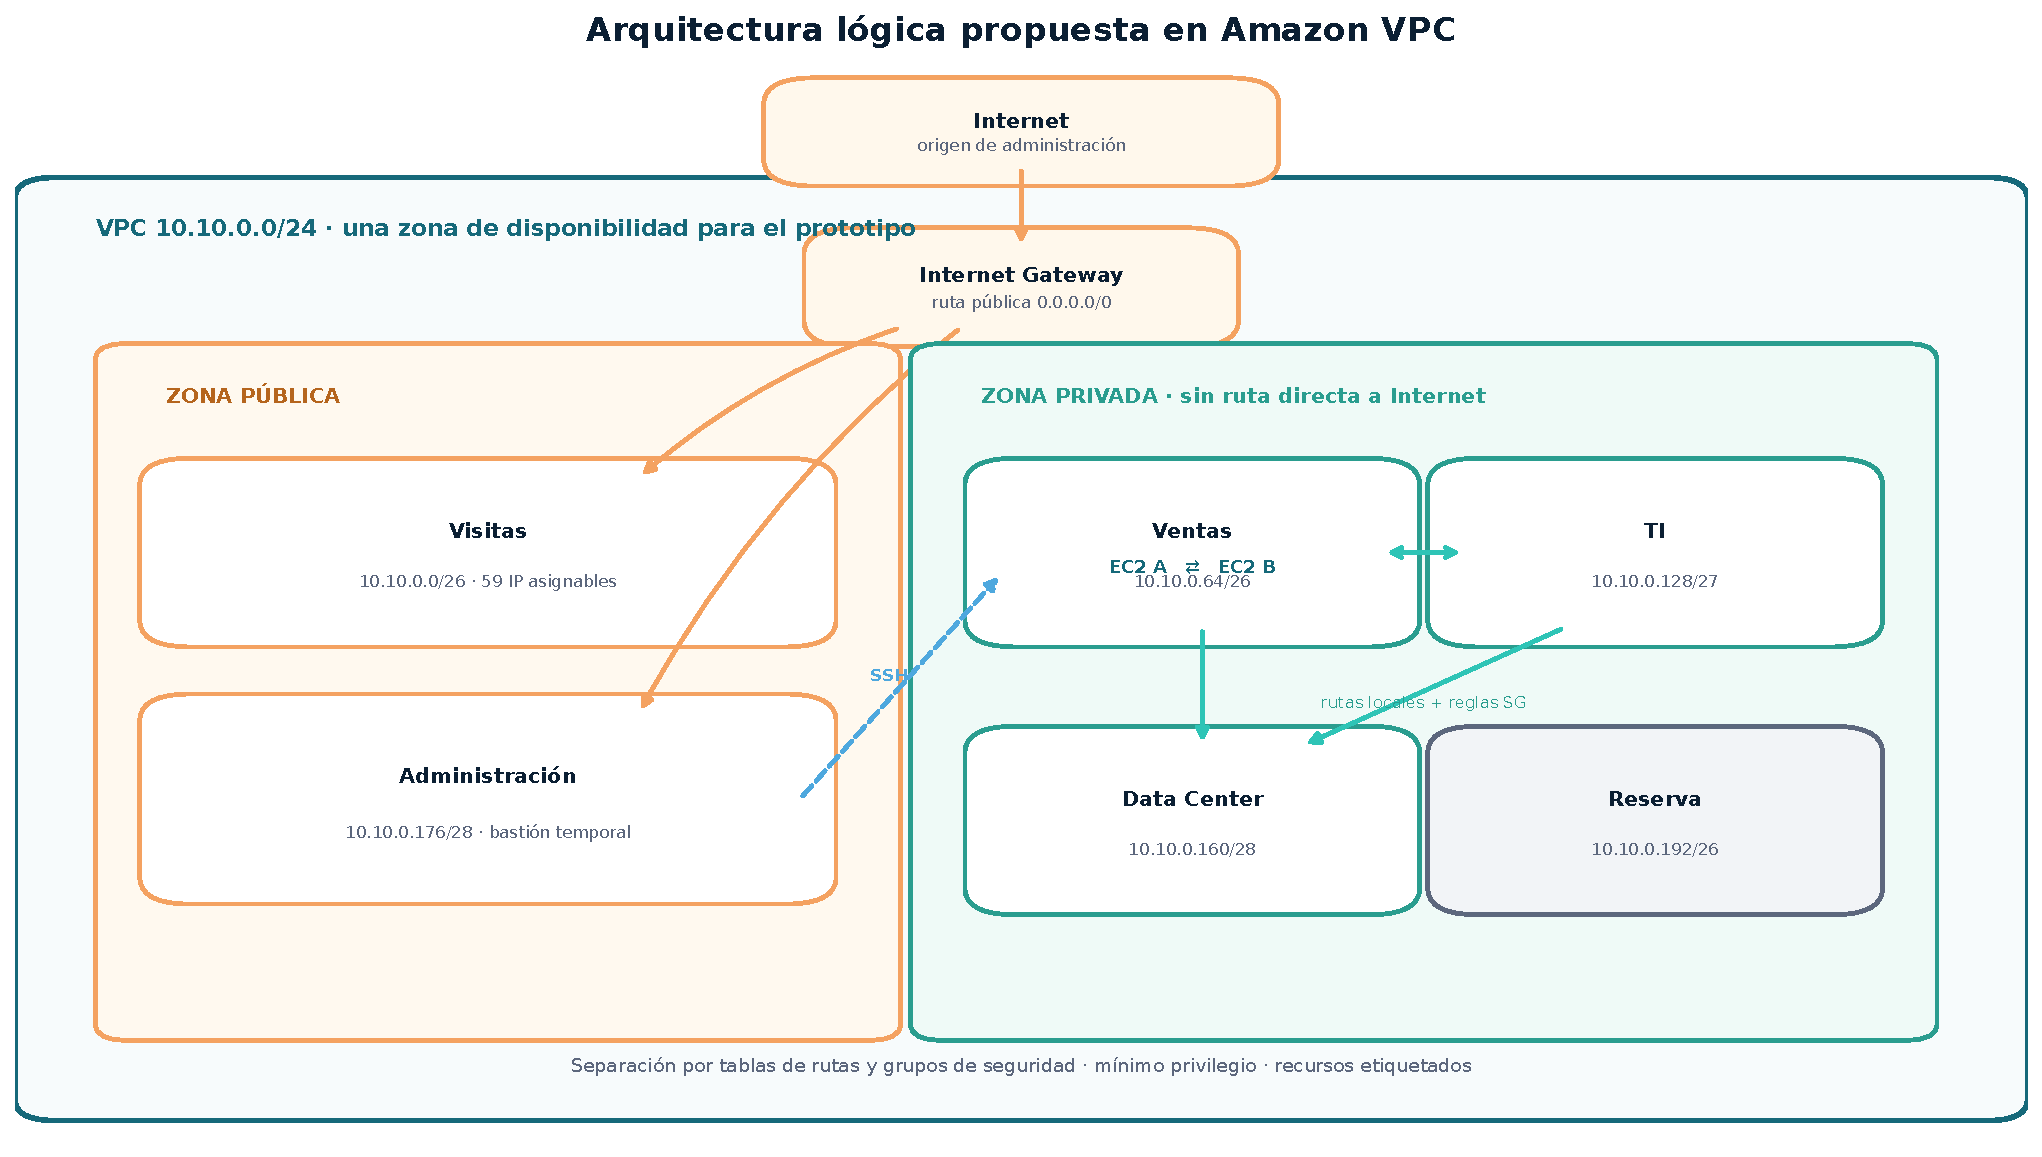
\includegraphics[width=\textwidth]{arquitectura-vpc.pdf}
\caption{Arquitectura lógica de la VPC propuesta. Elaboración propia.}
\label{fig:architecture}
\end{figure}

\section{Componentes}

\subsection{VPC}

La VPC habilita resolución y nombres DNS para facilitar una evolución posterior. Su tabla principal se mantiene sin rutas públicas adicionales. Esta decisión reduce el riesgo de que una subred creada en el futuro herede accidentalmente salida directa a Internet: las asociaciones con tablas personalizadas son explícitas.

\subsection{Subredes públicas}

Visitas y Administración se asocian con \code{public-rt}, que contiene la ruta local creada por AWS y \code{0.0.0.0/0} hacia el Internet Gateway. Ninguna de las dos habilita asignación automática de IP pública. De este modo, la clasificación ``pública'' depende del enrutamiento, pero cada recurso debe solicitar de forma deliberada una dirección pública.

Administración aloja únicamente el bastión temporal. Visitas se crea para demostrar la segmentación, pero la fase no ejecuta clientes invitados. En una ampliación real, sus dispositivos podrían acceder a Internet mediante un mecanismo diseñado para ese fin, manteniendo denegado el acceso a los segmentos internos.

\subsection{Subredes privadas}

Ventas, TI y Data Center se asocian con \code{private-rt}. La tabla sólo conserva la ruta \code{local} que AWS instala para el CIDR de la VPC. No se agrega NAT Gateway ni ruta a un Internet Gateway. Por tanto, las instancias de Ventas no pueden descargar paquetes desde Internet, pero sí intercambiar tráfico privado si los grupos de seguridad lo permiten.

\subsection{Bloque de reserva}

El bloque \code{10.10.0.192/26} no se declara como subred. Reservarlo permite incorporar posteriormente otra zona de disponibilidad, servicios compartidos o expansión departamental. Mantenerlo sin asignar evita asumir prematuramente su propósito y no consume recursos de AWS.

\section{Enrutamiento}

Cada subred debe estar asociada con una tabla de rutas, de manera explícita o implícita. Una tabla puede servir a varias subredes, pero cada subred sólo puede asociarse con una tabla a la vez \cite{aws-route-tables}. El prototipo aplica las siguientes decisiones:

\begin{table}[H]
\centering
\caption{Tablas de rutas propuestas}
\begin{tabularx}{\textwidth}{p{3.2cm}p{3.1cm}p{3.3cm}Y}
\toprule
\textbf{Tabla} & \textbf{Destino} & \textbf{Objetivo} & \textbf{Asociaciones} \\
\midrule
Pública & \code{10.10.0.0/24} & \code{local} & Visitas, Administración \\
Pública & \code{0.0.0.0/0} & Internet Gateway & Visitas, Administración \\
Privada & \code{10.10.0.0/24} & \code{local} & Ventas, TI, Data Center \\
\bottomrule
\end{tabularx}
\end{table}

AWS aplica coincidencia de prefijo más largo al elegir una ruta. La ruta local \code{/24} es más específica que \code{/0}; por ello el tráfico entre direcciones internas permanece dentro de la VPC. La ruta predeterminada sólo captura destinos no incluidos en el bloque local.

\section{Flujos representativos}

\subsection{Administración hacia Ventas}

El operador se conecta al bastión por SSH desde la única IP autorizada. Desde allí establece otro túnel SSH hacia la IP privada de la instancia de Ventas. El grupo de seguridad de Ventas no acepta SSH desde un CIDR arbitrario: referencia directamente el grupo de seguridad del bastión. Si la IP pública del operador cambia, se actualiza sólo \code{admin\_cidr}.

\subsection{Ventas hacia Ventas}

Las dos instancias comparten \code{ventas-sg}. Una regla ICMP con \code{self=true} acepta eco entre interfaces vinculadas al mismo grupo. El paquete se entrega por la ruta local y nunca sale hacia Internet. Éste es el flujo utilizado para la prueba de concepto.

\subsection{Visitas hacia redes internas}

La ruta local hace técnicamente alcanzables los prefijos de la VPC en la capa de enrutamiento, pero los grupos de seguridad de las cargas internas no contienen reglas que acepten tráfico originado por Visitas. En una versión productiva se complementaría este control con Network ACL o un firewall administrado si se requiere separación sin estado en el límite de subred.

\section{Escalabilidad}

El prototipo prioriza claridad y economía, no alta disponibilidad. Para producción se recomienda utilizar el bloque de reserva o ampliar el CIDR, duplicar subredes en otra zona y separar Administración de cualquier red de usuarios. También conviene reemplazar el bastión público por mecanismos administrados de acceso y añadir registros de flujo. Estas mejoras no alteran el aprendizaje central: los segmentos conservan prefijos distintos y políticas explícitas.

\chapter{Cálculos de subneteo}

\section{Fundamento}

Una dirección IPv4 contiene 32 bits. Un prefijo \code{/p} deja $h=32-p$ bits para identificar direcciones dentro de la subred. El tamaño total del bloque es:

\[
N_{\mathrm{total}} = 2^h = 2^{32-p}
\]

En una red tradicional suele enseñarse $N_{\mathrm{usable}}=2^h-2$ para descontar red y broadcast. AWS aplica una reserva distinta: las primeras cuatro direcciones y la última no pueden asignarse a una interfaz. Por tanto:

\[
N_{\mathrm{AWS}} = 2^{32-p}-5
\]

El número mínimo de bits de host para una demanda $H$ cumple:

\[
2^h-5 \geq H
\qquad\Longrightarrow\qquad
h=\left\lceil\log_2(H+5)\right\rceil,
\quad p=32-h
\]

Además de satisfacer la desigualdad, AWS impone \code{/28} como la subred IPv4 más pequeña permitida \cite{aws-subnet-sizing}. Todas las selecciones siguientes respetan ambos límites.

\section{Cálculo de Visitas}

El enunciado no fija cantidad, por lo que se declara $H=30$ visitantes concurrentes:

\[
h=\left\lceil\log_2(30+5)\right\rceil
=\left\lceil\log_2(35)\right\rceil
=\lceil5.13\rceil=6
\]

\[
p=32-6=26,\qquad
N_{\mathrm{total}}=2^6=64,\qquad
N_{\mathrm{AWS}}=64-5=59
\]

Se asigna \code{10.10.0.0/26}, máscara \code{255.255.255.192}. El tamaño de bloque en el último octeto es $256-192=64$. La red inicia en .0 y termina en .63. AWS reserva .0, .1, .2, .3 y .63; el rango asignable es .4--.62. La ocupación inicial prevista es $30/59=50.85\%$.

\section{Cálculo de Ventas}

Para $H=25$:

\[
h=\left\lceil\log_2(25+5)\right\rceil
=\left\lceil\log_2(30)\right\rceil=5,
\quad p=27
\]

El mínimo matemático es \code{/27}: $2^5-5=27$ direcciones asignables. Sin embargo, después de asignar una dirección a cada persona quedarían sólo dos. La holgura sería:

\[
\frac{27-25}{27}\times100=7.41\%
\]

Esta reserva es insuficiente si cada colaborador usa más de un dispositivo o si aparecen interfaces de servicios. Se selecciona operativamente \code{/26}:

\[
N_{\mathrm{AWS}}=2^6-5=59,qquad
\text{ocupación}=\frac{25}{59}\times100=42.37\%
\]

La subred es \code{10.10.0.64/26}. Su intervalo completo es .64--.127; AWS reserva .64--.67 y .127; el rango asignable es .68--.126. Esta decisión distingue el valor mínimo del valor recomendado y documenta el costo de la holgura.

\section{Cálculo de TI}

Para $H=15$:

\[
h=\left\lceil\log_2(15+5)\right\rceil
=\left\lceil\log_2(20)\right\rceil=5,
\qquad p=27
\]

Un \code{/28} tendría 16 direcciones totales y sólo 11 asignables en AWS, por lo que no cumple. Con \code{/27}, TI obtiene 27 asignables y 12 libres. Se asigna \code{10.10.0.128/27}, máscara \code{255.255.255.224} e incremento $256-224=32$. El bloque completo va de .128 a .159 y el rango asignable de .132 a .158.

\section{Cálculo de Data Center}

Para $H=5$:

\[
h=\left\lceil\log_2(5+5)\right\rceil
=\left\lceil\log_2(10)\right\rceil=4,
\qquad p=28
\]

La subred elegida es \code{10.10.0.160/28}. Contiene 16 direcciones y 11 asignables. Su máscara es \code{255.255.255.240} y el incremento es 16. AWS reserva .160--.163 y .175; los servidores pueden utilizar .164--.174. La capacidad libre es seis direcciones, equivalente al 54.55\% del espacio asignable.

\section{Cálculo de Administración}

El prototipo requiere un bastión y admite hasta tres componentes administrativos. Un bloque menor podría parecer suficiente matemáticamente. Sin embargo, AWS no permite subredes IPv4 más pequeñas que \code{/28}. Se asigna \code{10.10.0.176/28}. El intervalo completo es .176--.191, las direcciones reservadas son .176--.179 y .191, y el rango asignable es .180--.190.

\section{Resumen detallado}

\small
\begin{longtable}{p{2.4cm}p{2.8cm}p{2.3cm}p{2.9cm}p{2.5cm}}
\caption{Plan de direccionamiento IPv4}\label{tab:addressing}\\
\toprule
\textbf{Segmento} & \textbf{CIDR / máscara} & \textbf{Bloque completo} & \textbf{Reservas AWS} & \textbf{Asignables} \\
\midrule
\endfirsthead
\toprule
\textbf{Segmento} & \textbf{CIDR / máscara} & \textbf{Bloque completo} & \textbf{Reservas AWS} & \textbf{Asignables} \\
\midrule
\endhead
Visitas & \code{10.10.0.0/26} \newline 255.255.255.192 & .0--.63 & .0, .1, .2, .3, .63 & .4--.62 (59) \\
Ventas & \code{10.10.0.64/26} \newline 255.255.255.192 & .64--.127 & .64, .65, .66, .67, .127 & .68--.126 (59) \\
TI & \code{10.10.0.128/27} \newline 255.255.255.224 & .128--.159 & .128, .129, .130, .131, .159 & .132--.158 (27) \\
Data Center & \code{10.10.0.160/28} \newline 255.255.255.240 & .160--.175 & .160, .161, .162, .163, .175 & .164--.174 (11) \\
Administración & \code{10.10.0.176/28} \newline 255.255.255.240 & .176--.191 & .176, .177, .178, .179, .191 & .180--.190 (11) \\
Reserva & \code{10.10.0.192/26} \newline 255.255.255.192 & .192--.255 & No aplica hasta crear subred & 64 sin asignar \\
\bottomrule
\end{longtable}
\normalsize

\begin{figure}[H]
\centering
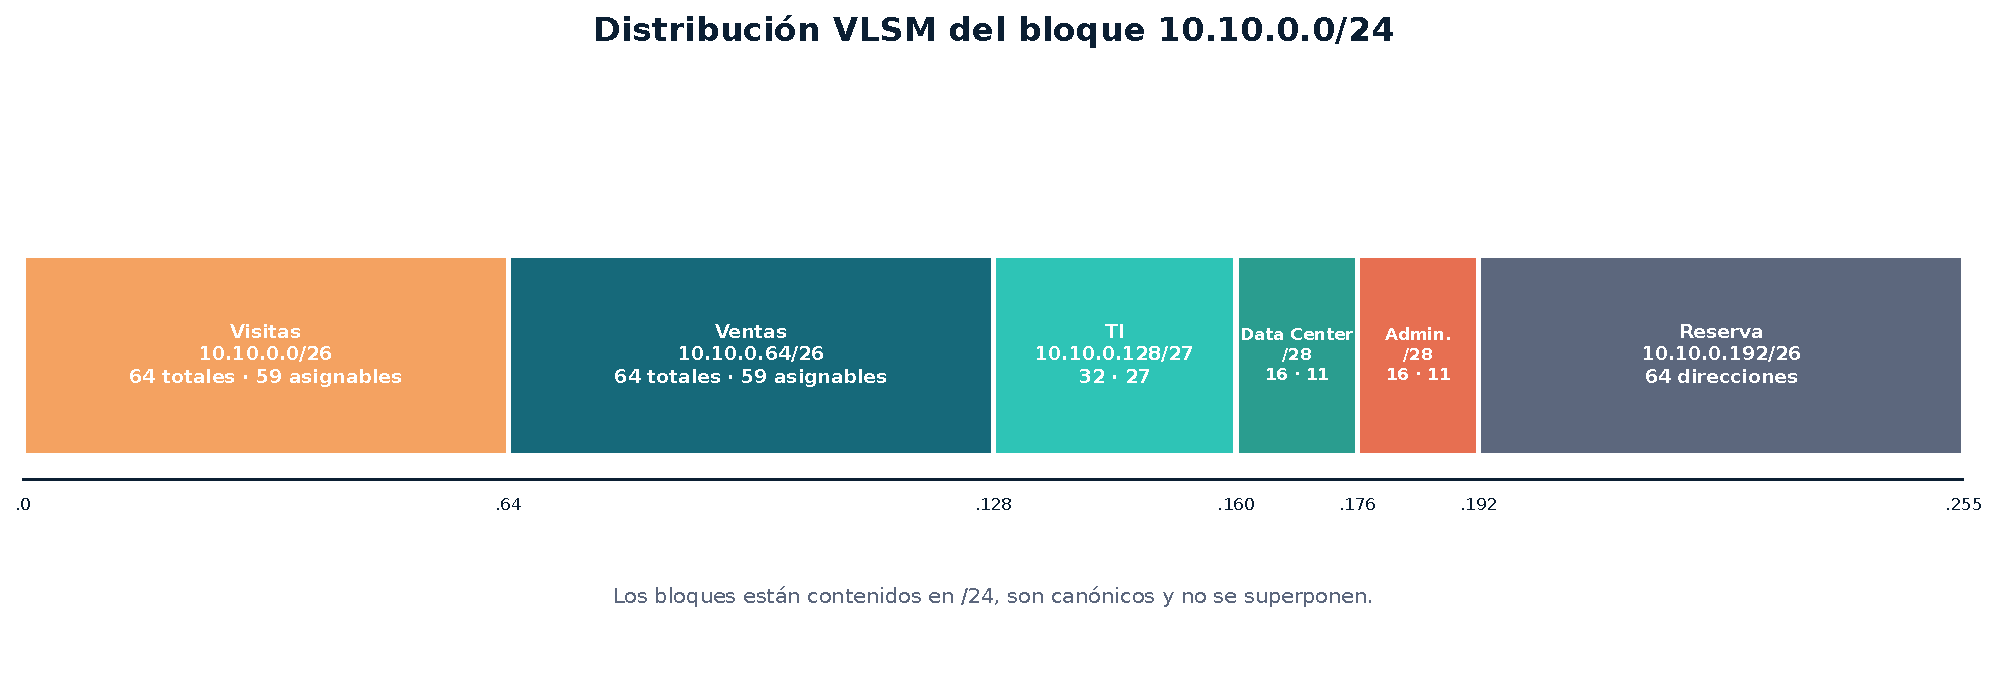
\includegraphics[width=\textwidth]{mapa-cidr.pdf}
\caption{Mapa proporcional del espacio de direcciones. Elaboración propia.}
\label{fig:cidr-map}
\end{figure}

\section{Demostración de contención y no solapamiento}

Los límites aparecen en múltiplos correctos de sus tamaños: 0 y 64 para bloques de 64; 128 para el bloque de 32; 160 y 176 para bloques de 16; y 192 para el bloque final de 64. Cada inicio coincide con el final anterior más uno. La suma es:

\[
64+64+32+16+16+64=256=2^8
\]

Por lo tanto, el plan cubre exactamente el \code{/24} sin huecos ni intersecciones. El script \path{scripts/validate-network.py} reproduce esta comprobación con la biblioteca estándar de Python. Su salida se conserva en \path{evidence/deployment/cidr-validation.txt}.

\chapter{Segmentación, seguridad y rutas}

\section{Modelo de confianza}

La segmentación no se limita a asignar prefijos diferentes. Dentro de una VPC existe una ruta local que puede transportar paquetes entre subredes. El aislamiento efectivo surge de combinar direccionamiento, tablas de rutas, direcciones públicas y grupos de seguridad. La política adoptada es denegar por defecto y habilitar sólo flujos relacionados con la prueba o la administración.

\begin{figure}[H]
\centering
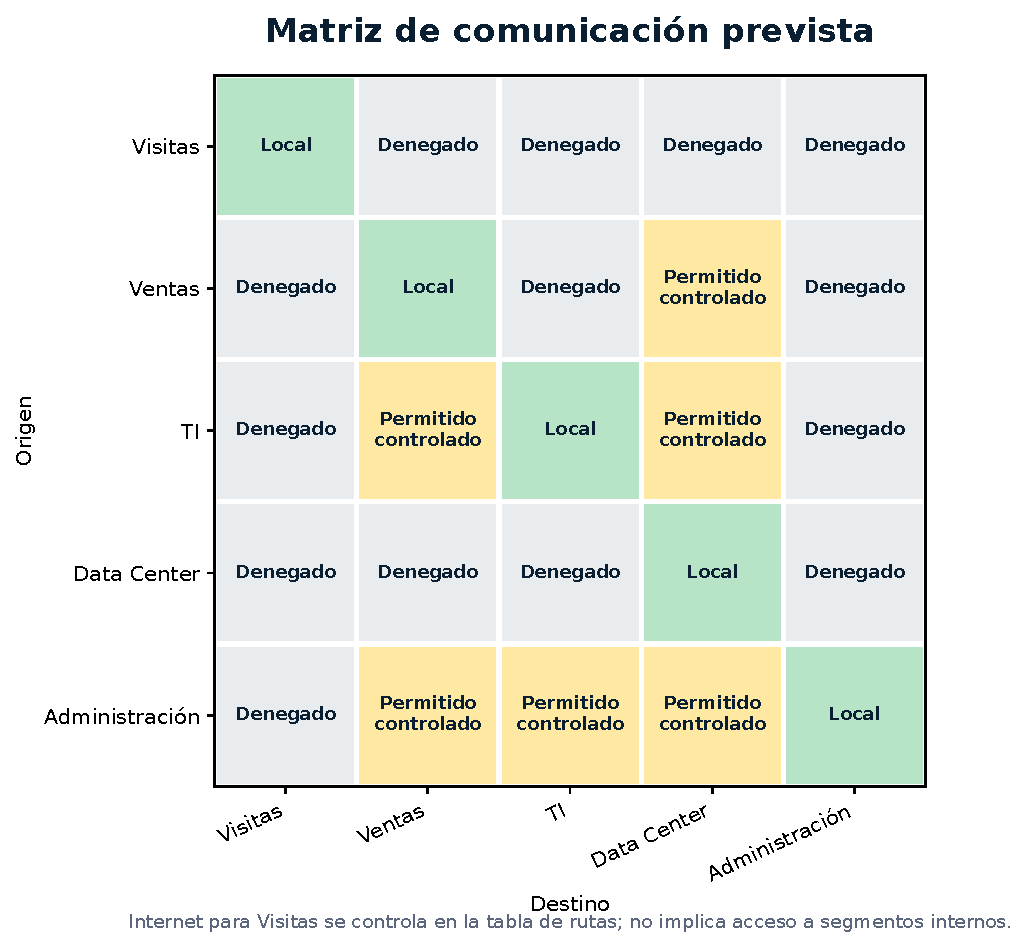
\includegraphics[width=0.83\textwidth]{matriz-seguridad.pdf}
\caption{Matriz de comunicación prevista entre segmentos. Elaboración propia.}
\label{fig:security-matrix}
\end{figure}

\section{Grupos de seguridad}

\subsection{Grupo del bastión}

La entrada TCP/22 se restringe a \code{admin\_cidr}, que debe ser una dirección IPv4 con prefijo \code{/32}. La validación de Terraform rechaza valores que no cumplan ese formato. La salida se limita al CIDR de la VPC; el bastión no necesita acceso general a Internet para ejecutar la prueba.

\subsection{Grupo de Ventas}

SSH sólo se acepta desde interfaces que pertenezcan al grupo del bastión. Esta referencia es más estable que escribir la IP privada del bastión. ICMP se acepta cuando origen y destino utilizan el mismo grupo de Ventas. La salida también se limita al \code{/24}. No existen reglas de entrada desde Visitas, Internet o un rango general.

\begin{table}[H]
\centering
\caption{Reglas relevantes del prototipo}
\begin{tabularx}{\textwidth}{p{2.7cm}p{2.0cm}p{2.2cm}Y}
\toprule
\textbf{Grupo} & \textbf{Dirección} & \textbf{Protocolo} & \textbf{Origen o destino} \\
\midrule
Bastión & Entrada & TCP/22 & IP administrativa \code{/32} \\
Bastión & Salida & Todos & \code{10.10.0.0/24} \\
Ventas & Entrada & TCP/22 & Grupo de seguridad del bastión \\
Ventas & Entrada & ICMP & El mismo grupo de seguridad \\
Ventas & Salida & Todos & \code{10.10.0.0/24} \\
\bottomrule
\end{tabularx}
\end{table}

\section{Defensa en profundidad}

Los volúmenes raíz se cifran y las instancias exigen tokens de Instance Metadata Service versión 2. No se versionan llaves privadas ni archivos de estado. El archivo \code{.gitignore} excluye \code{*.pem}, \code{*.key}, \code{terraform.tfvars}, \code{*.tfstate} y la carpeta de trabajo del proveedor.

El prototipo no agrega Network ACL personalizadas porque los grupos con estado bastan para demostrar la política y reducen el riesgo de bloquear respuestas efímeras. En producción, una ACL o firewall puede complementar el control cuando la organización necesite reglas sin estado a nivel de subred, inspección o evidencia centralizada.

\section{Amenazas operativas y controles}

\begin{longtable}{p{4.0cm}p{5.0cm}p{4.4cm}}
\toprule
\textbf{Riesgo} & \textbf{Consecuencia} & \textbf{Control} \\
\midrule
\endfirsthead
\toprule
\textbf{Riesgo} & \textbf{Consecuencia} & \textbf{Control} \\
\midrule
\endhead
SSH abierto al mundo & Intentos de acceso y exposición innecesaria. & Validación obligatoria de \code{admin\_cidr /32}. \\
Llave privada en Git & Compromiso de instancias y persistencia del secreto. & Exclusión por extensión; sólo se declara la ruta a la llave pública. \\
Instancias privadas con IP pública & Ruptura del modelo de exposición. & \code{associate\_public\_ip\_} \newline \code{address=false}. \\
Uso de metadatos sin token & Mayor exposición ante ciertas solicitudes inducidas. & IMDSv2 obligatorio. \\
Recursos olvidados & Cargos posteriores a la entrega. & Etiqueta de expiración y destrucción automatizada. \\
Permisos IAM excesivos & Daño más allá del proyecto. & Usar identidad académica separada y permisos limitados. \\
Solapamiento CIDR & Rutas ambiguas y fallas de creación. & Validación local y validación del proveedor. \\
\bottomrule
\end{longtable}

\section{Limitaciones de seguridad}

Una prueba exitosa de ping sólo confirma alcance ICMP entre dos interfaces bajo las reglas presentes. No demuestra confidencialidad del tráfico, seguridad de aplicaciones, resistencia a ataques o disponibilidad. La fase tampoco valida identidad de usuarios finales. Estas propiedades exigirían controles adicionales y pruebas específicas.

\chapter{Implementación del prototipo}

\section{Estrategia reproducible}

La implementación se define en \code{infra/terraform}. En lugar de crear recursos manualmente y depender de memoria o capturas aisladas, el equipo conserva una descripción declarativa. Terraform compara esa descripción con el proveedor y presenta un plan antes de realizar cambios. La separación de archivos no altera el resultado, pero facilita la revisión: \code{network.tf} contiene VPC, subredes y rutas; \code{security.tf} contiene políticas; y \code{compute.tf} contiene recursos temporales.

\begin{figure}[H]
\centering
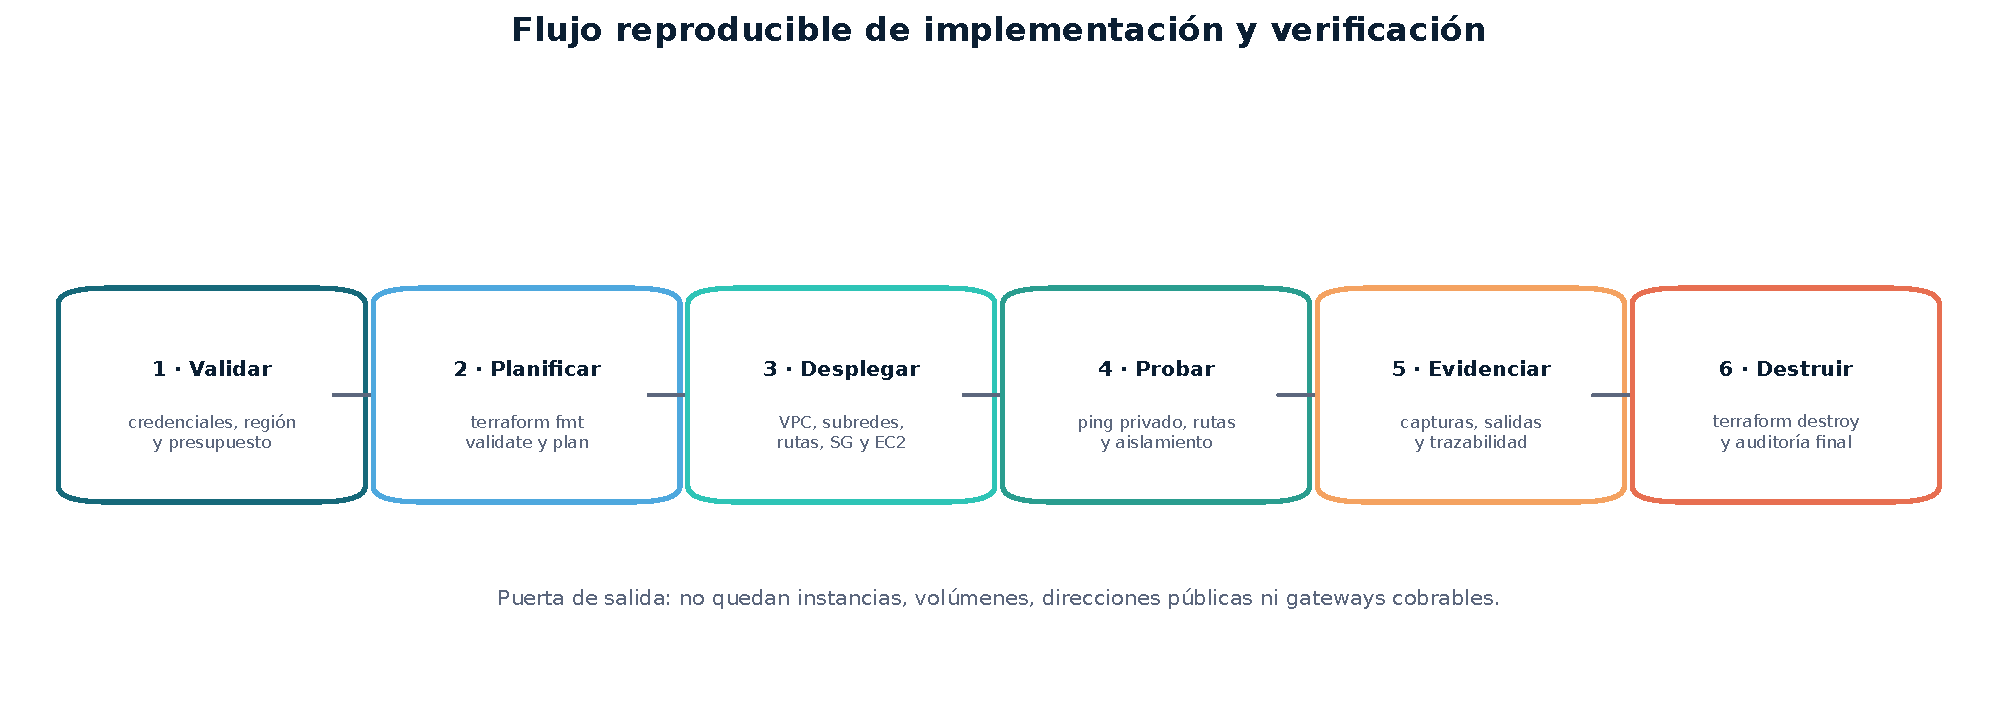
\includegraphics[width=\textwidth]{flujo-implementacion.pdf}
\caption{Flujo controlado para implementar, evidenciar y destruir. Elaboración propia.}
\label{fig:workflow}
\end{figure}

\section{Preparación}

\subsection{Identidad y región}

La identidad AWS debe pertenecer a una cuenta autorizada por el equipo. No se aceptan credenciales escritas dentro de archivos Terraform ni almacenadas en el repositorio. Antes de desplegar se verifica la identidad con un mecanismo de autenticación local, se confirma la región y se revisan los límites de servicio. La variable predeterminada es \code{us-east-1}, pero puede cambiarse sin alterar los CIDR.

El 20 de octubre de 2026 se verificó una sesión activa mediante \code{aws sts get-caller-identity} y se confirmó el perfil configurado en \code{us-east-1}. La Figura~\ref{fig:aws-identity-region} conserva los identificadores sensibles parcialmente ocultos y no muestra claves, tokens ni contraseñas.

\begin{figure}[H]
\centering
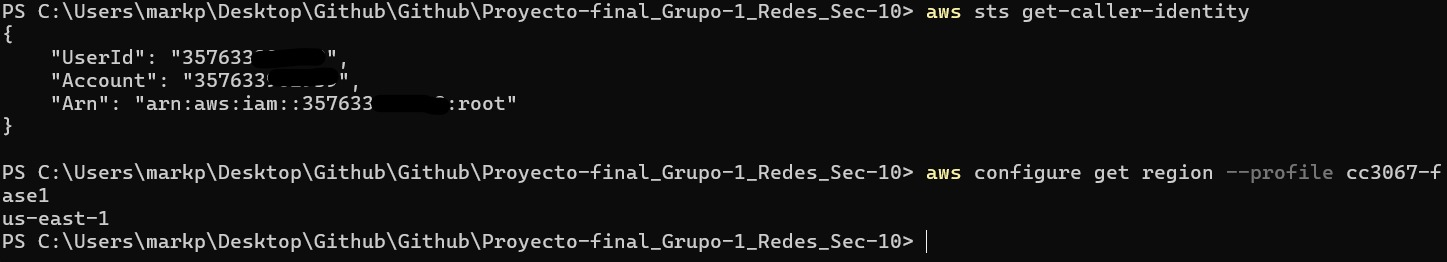
\includegraphics[width=0.96\textwidth]{aws-identidad-region-us-east-1.jpeg}
\caption{Verificación genuina de identidad AWS y región configurada. Los identificadores de cuenta fueron redactados antes de incorporarlos al informe.}
\label{fig:aws-identity-region}
\end{figure}

\begin{warningbox}[Control de privilegios]
La salida capturada identifica al principal raíz de la cuenta. Esta evidencia confirma acceso, pero no justifica usar privilegios raíz durante el despliegue. En la ventana de implementación debe preferirse un rol o usuario temporal con permisos limitados a los recursos del laboratorio.
\end{warningbox}

\subsection{Llave temporal}

La prueba necesita una llave SSH sólo durante la ventana de ejecución. El equipo genera el par fuera del repositorio, entrega a Terraform únicamente la ruta de la parte pública y protege la parte privada. Al destruir el entorno se elimina el recurso \code{aws\_key\_pair}; el archivo privado local se elimina mediante un procedimiento controlado después de verificar que ya no se necesita.

\subsection{Variables}

El archivo \code{terraform.tfvars.example} sirve de plantilla. \code{admin\_cidr} debe sustituirse por la IPv4 pública del operador con \code{/32}; \code{public\_key\_path} apunta a la llave pública temporal; y \code{enable\_compute=true} activa las tres instancias. El valor predeterminado es \code{false}, por lo que un uso descuidado no crea cómputo.

\section{Creación de la red}

La secuencia lógica es la siguiente:

\begin{enumerate}
  \item El proveedor consulta zonas disponibles y la AMI más reciente de Amazon Linux 2023.
  \item Se crea la VPC \code{10.10.0.0/24}, con DNS habilitado.
  \item Se crea un Internet Gateway y se adjunta a la VPC.
  \item Se crean cinco subredes canónicas en la primera zona disponible.
  \item Se crea una tabla pública con \code{0.0.0.0/0} hacia el gateway.
  \item Se crea una tabla privada sin salida predeterminada.
  \item Visitas y Administración se asocian con la tabla pública.
  \item Ventas, TI y Data Center se asocian con la tabla privada.
\end{enumerate}

Una tabla pública no asigna por sí sola direcciones públicas. La asignación automática mediante \path{map_public_ip_on_launch} permanece desactivada en todas las subredes. Únicamente el recurso del bastión solicita una dirección pública de manera explícita.

\section{Aplicación de seguridad}

Terraform crea dos grupos. El primero permite SSH desde la IP administrativa y salida sólo dentro de la VPC. El segundo permite SSH desde el grupo del bastión e ICMP entre sus propios miembros. Las dependencias se infieren a partir de las referencias entre recursos; por ejemplo, Ventas utiliza el identificador del grupo del bastión, no una cadena escrita manualmente.

\section{Creación del cómputo}

Con \code{enable\_compute=true}, se registra la llave pública, se crea un bastión en Administración y dos instancias en Ventas. Las tres usan volúmenes raíz GP3 de 8 GiB cifrados. El bastión recibe IP pública; las dos instancias de Ventas sólo reciben IP privadas. Las salidas de Terraform muestran la IP del bastión y la lista de IP privadas sin revelar secretos.

\section{Comandos de ejecución previstos}

\begin{Verbatim}[fontsize=\small,frame=single]
terraform init
terraform fmt -check -recursive
terraform validate
terraform plan -out=tfplan
terraform apply tfplan

# Después de capturar la evidencia:
terraform destroy
\end{Verbatim}

\begin{warningbox}[Nota sobre la ejecución final y el control de costos]
Las capturas incorporadas en esta versión demuestran que existe una identidad AWS configurada y que Terraform puede generar el plan de creación esperado. El equipo detuvo deliberadamente el procedimiento antes de \code{terraform apply} para evitar cargos por instancias EC2, almacenamiento y dirección IPv4 pública fuera de la ventana definitiva de pruebas.

La implementación real se realizará al final del proyecto, dentro de una única ventana corta y supervisada. En esa misma sesión se aplicará el plan, se capturarán la VPC, las subredes, las tablas de rutas, los grupos de seguridad y las instancias; se ejecutará el ping entre las dos instancias privadas de Ventas; y se destruirán todos los recursos inmediatamente después de conservar la evidencia. Por tanto, estas actividades representan compromisos de ejecución final y no resultados ya obtenidos.
\end{warningbox}

\chapter{Plan y resultados de pruebas}

\section{Principio de verificación}

Cada prueba define precondición, acción, resultado esperado y evidencia. Esta estructura impide confundir una intención de diseño con un resultado observado. Las pruebas locales se ejecutaron sobre los archivos versionados. La evidencia del 22 de octubre de 2026 demuestra también el despliegue en AWS y las dos pruebas de conectividad. Los cinco controles definidos para el alcance de la Fase 1 están verificados.

\section{Prueba P-01: capacidad y no solapamiento}

\textbf{Precondición:} Python 3 disponible.

\textbf{Acción:} ejecutar \code{python scripts/validate-network.py}.

\textbf{Criterios:} todas las subredes deben pertenecer al \code{/24}; ninguna puede superponerse; $2^{32-p}-5$ debe cubrir la demanda; el bloque de reserva no debe intersectar una subred activa.

\textbf{Resultado:} \statusok. La suma de bloques es 256, todos los comienzos son canónicos y cada capacidad supera la demanda declarada. La salida completa se conserva como texto UTF-8.

\section{Prueba P-02: formato y validez de Terraform}

\textbf{Precondición:} Terraform y el proveedor oficial de AWS inicializados.

\textbf{Acción:} ejecutar \code{terraform fmt -check -recursive} y \code{terraform validate -no-color}.

\textbf{Criterio:} el formateador no propone cambios y la validación finaliza con código cero.

\textbf{Resultado:} \statusok. La salida registrada indica: ``Success! The configuration is valid.''

\begin{figure}[H]
\centering
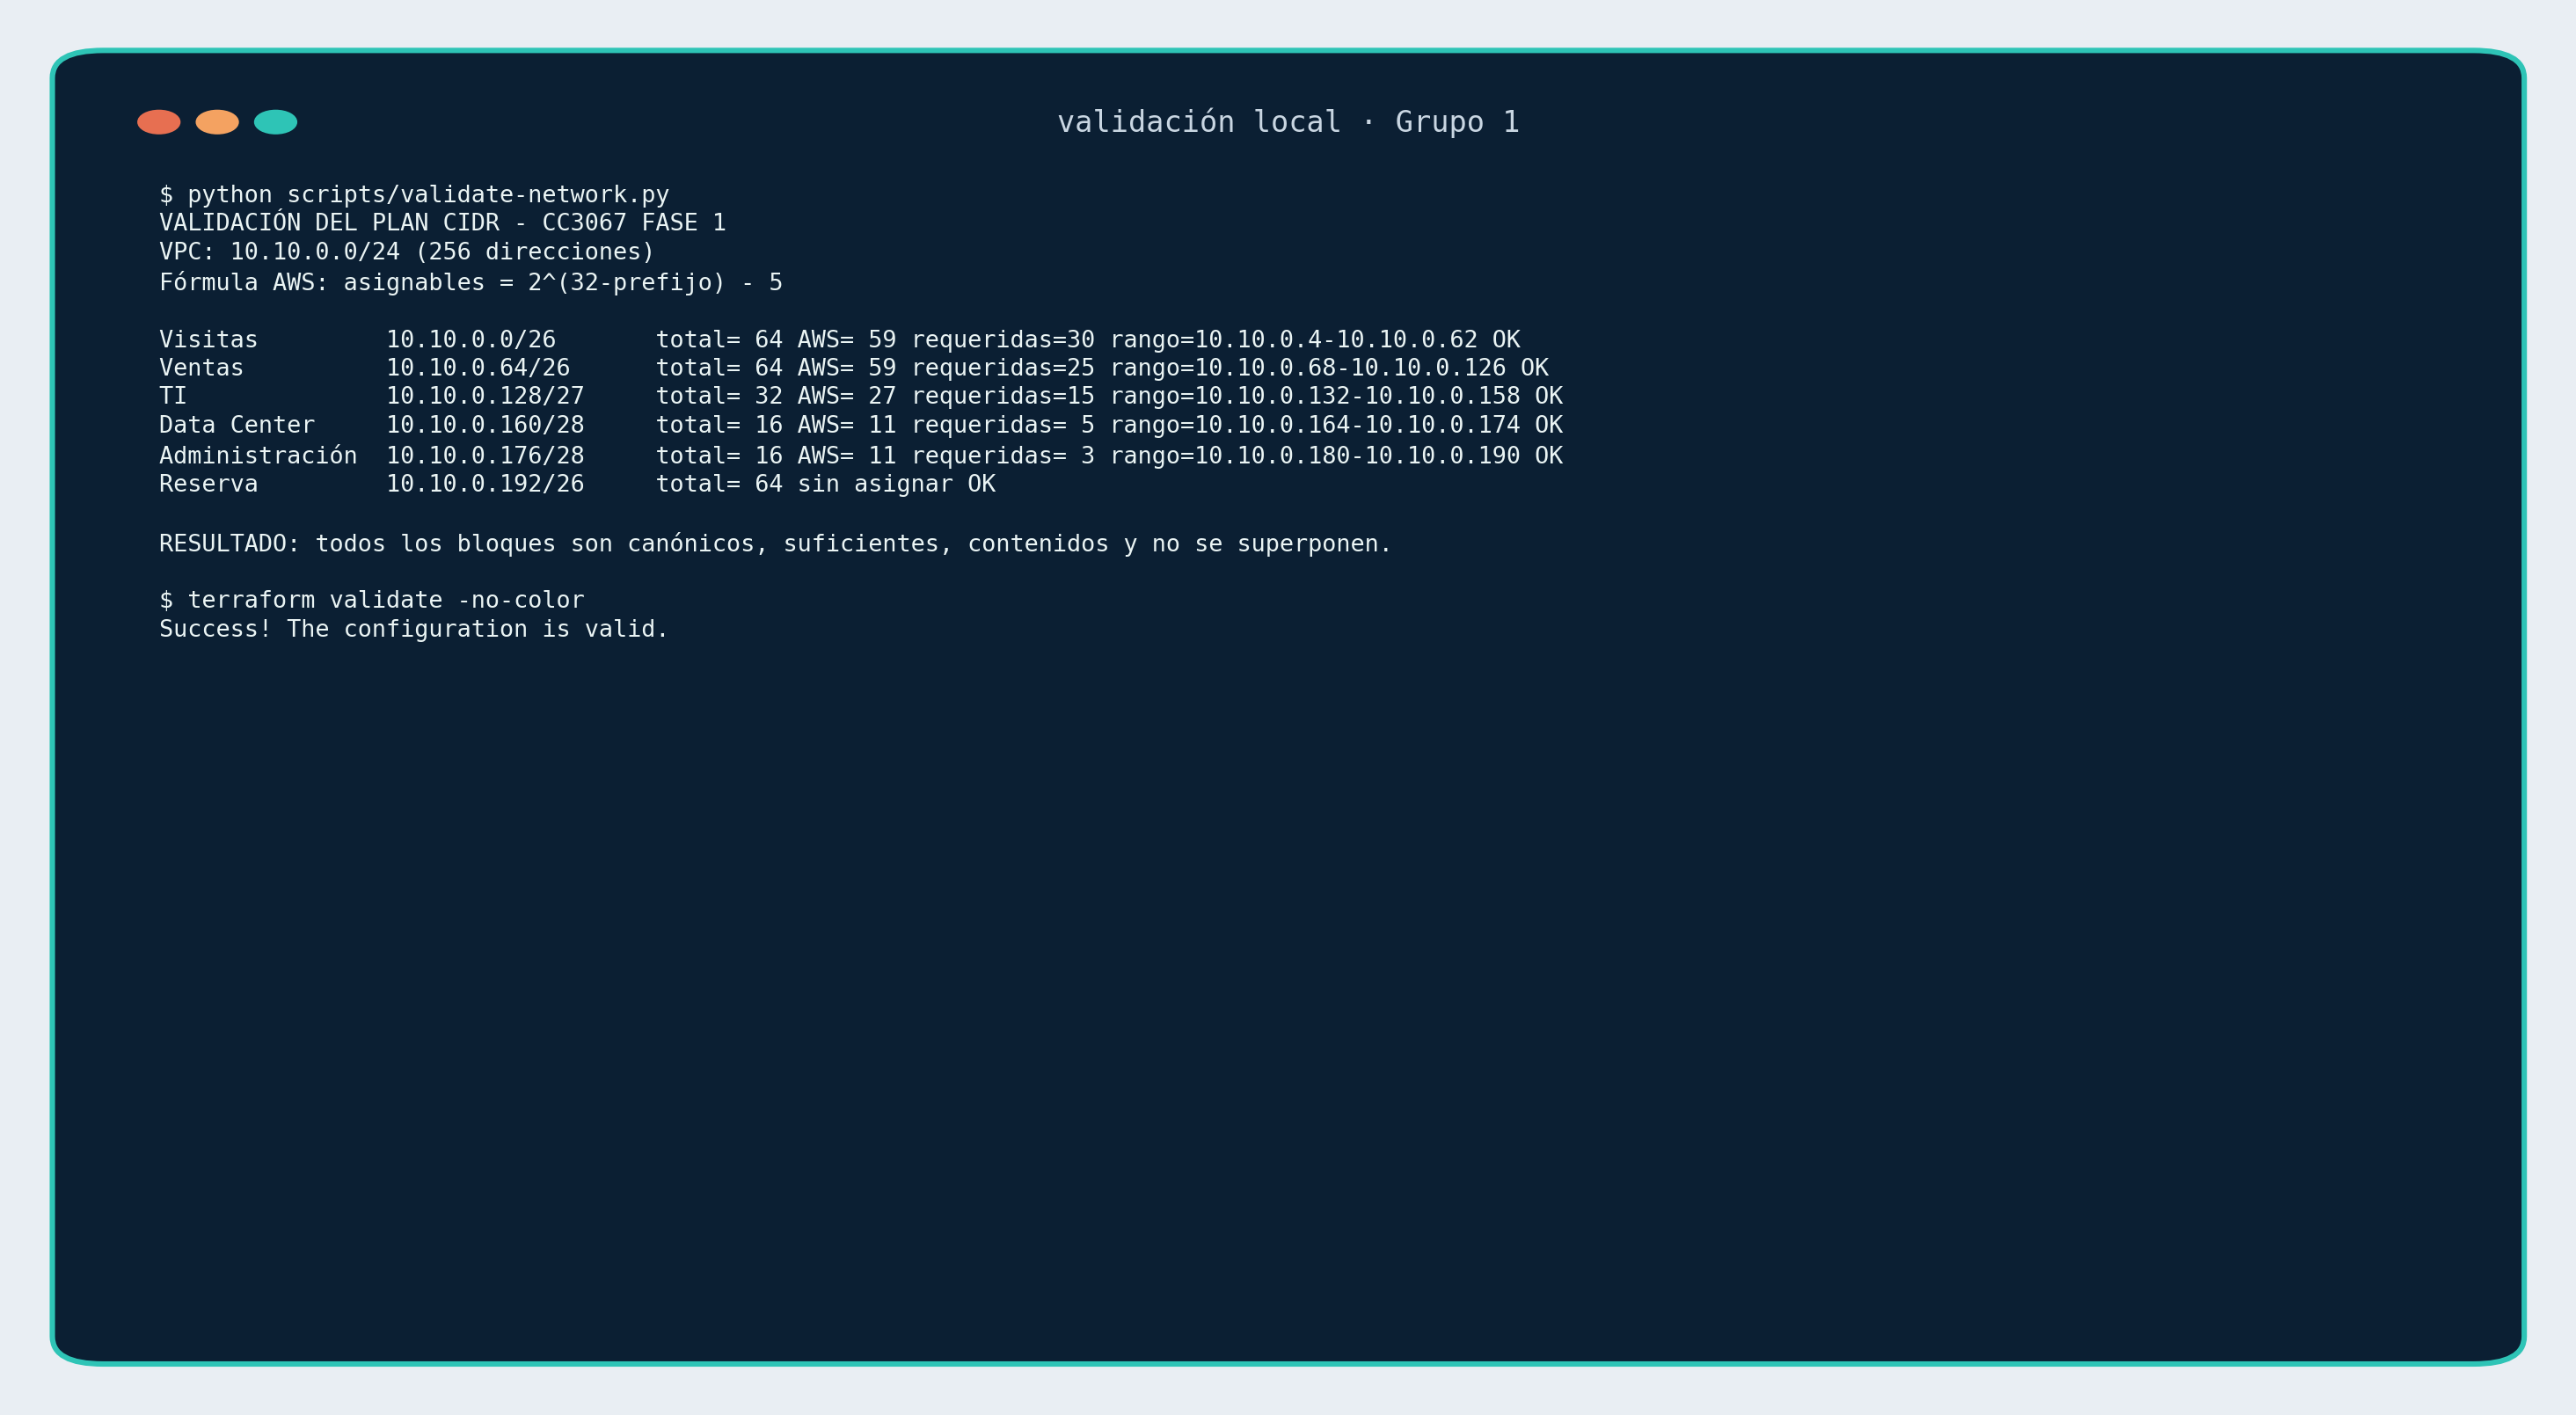
\includegraphics[width=0.93\textwidth]{validacion-local.png}
\caption{Captura reproducible de las validaciones locales.}
\label{fig:local-validation}
\end{figure}

\section{Prueba P-03: planificación contra el proveedor}

\textbf{Precondición:} credenciales AWS configuradas mediante un mecanismo admitido por el proveedor.

\textbf{Acción:} ejecutar \code{terraform plan} primero con cómputo deshabilitado y luego con las variables de prueba.

\textbf{Criterio:} el plan reconoce la identidad, consulta zona y AMI, y propone exclusivamente los recursos documentados.

\textbf{Resultado actual:} \statusok. La identidad AWS fue reconocida, la región se confirmó como \code{us-east-1} y Terraform produjo un plan compuesto únicamente por altas previstas. La Figura~\ref{fig:terraform-cloud-plan} muestra recursos para la VPC, cinco subredes, tablas y asociaciones de rutas, grupos de seguridad, llave temporal, bastión y dos instancias de Ventas.

\begin{figure}[H]
\centering
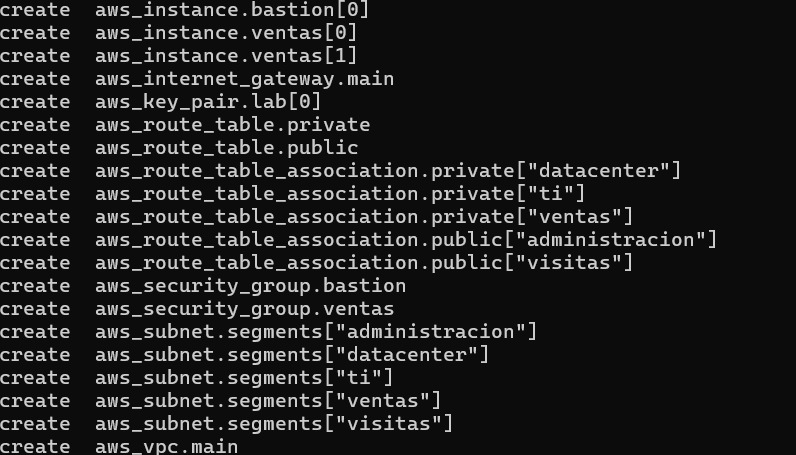
\includegraphics[width=0.96\textwidth]{terraform-plan-recursos-previstos.jpeg}
\caption{Evidencia genuina del plan Terraform contra AWS. Esta captura documenta la revisión previa al \code{apply}; la ejecución real se acredita por separado.}
\label{fig:terraform-cloud-plan}
\end{figure}

Esta prueba verifica autenticación y planificación contra el proveedor. La existencia posterior de la infraestructura no se infiere del plan: se demuestra mediante la salida real de \code{terraform apply}, los identificadores observados y las capturas de la Figura~\ref{fig:aws-deployment-real}.

\section{Prueba P-04: conectividad privada}

\textbf{Precondición:} bastión y dos instancias de Ventas en estado \emph{running}; llaves y reglas activas.

\textbf{Acción:} desde la instancia Ventas A ejecutar:

\begin{Verbatim}[fontsize=\small,frame=single]
ping -c 4 <IP_PRIVADA_VENTAS_B>
\end{Verbatim}

El script \code{scripts/test-connectivity.ps1} utiliza SSH con salto por el bastión, registra origen, destino, fecha y salida, y guarda \code{evidence/connectivity/ping-private.txt}.

\textbf{Criterio:} cuatro paquetes transmitidos, cuatro recibidos y 0\% de pérdida. Las dos direcciones deben pertenecer a \code{10.10.0.64/26}; ninguna debe ser pública.

\textbf{Resultado:} \statusok. Desde \code{10.10.0.71} se enviaron cuatro paquetes a \code{10.10.0.79}; se recibieron los cuatro y se observó 0\% de pérdida. Ambas direcciones pertenecen a la subred de Ventas \code{10.10.0.64/26}. El siguiente extracto proviene del registro genuino conservado en el repositorio:

\VerbatimInput[fontsize=\footnotesize,frame=single,firstline=7,lastline=15]{../../evidence/connectivity/ping-private.txt}

\section{Prueba P-05: aislamiento}

Después del ping exitoso, se intenta ICMP desde el bastión hacia una instancia de Ventas. La regla de Ventas acepta ICMP sólo desde su propio grupo, por lo que el tráfico del bastión debe fallar. Esta prueba negativa demuestra que permitir administración SSH no equivale a permitir todo protocolo.

\textbf{Resultado:} \statusok. El bastión intentó alcanzar \code{10.10.0.71}; se transmitieron cuatro paquetes, ninguno fue recibido y la pérdida fue 100\%. El resultado es coherente con la regla que acepta ICMP sólo entre miembros del grupo de Ventas.

\begin{figure}[H]
\centering
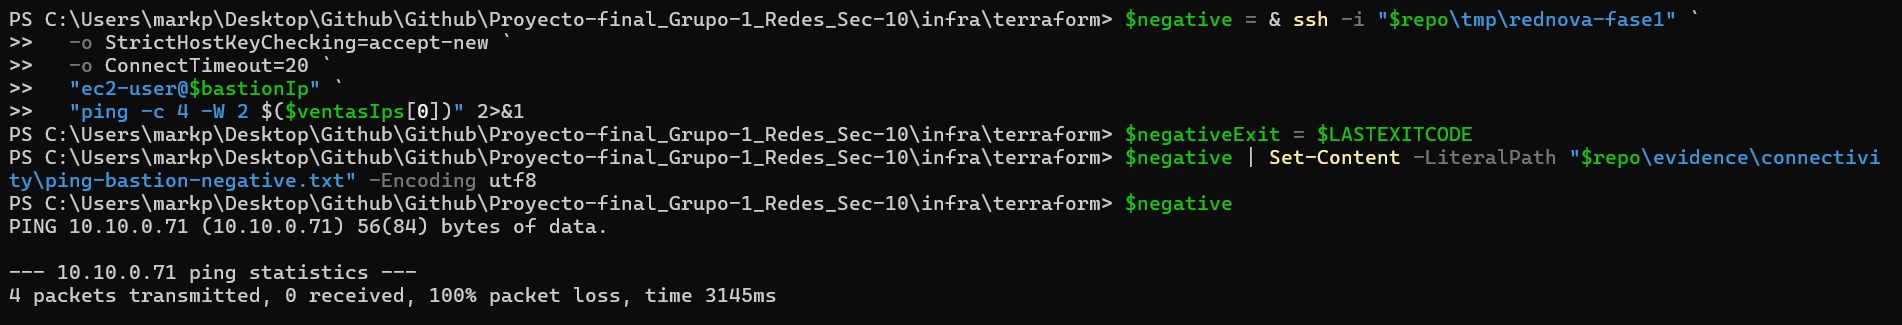
\includegraphics[width=0.94\textwidth]{04-prueba-icmp-bastion-bloqueada.png}
\caption{Prueba genuina de aislamiento: ICMP desde el bastión hacia Ventas fue bloqueado.}
\label{fig:bastion-negative-test}
\end{figure}

\section{Matriz de resultados}

\begin{table}[H]
\centering
\caption{Resumen de verificación}
\begin{tabularx}{\textwidth}{p{1.6cm}Y p{3.4cm}}
\toprule
\textbf{Prueba} & \textbf{Propiedad observada} & \textbf{Estado} \\
\midrule
P-01 & Capacidad, contención, canonicidad y no solapamiento. & \statusok \\
P-02 & Sintaxis, formato y relaciones del código Terraform. & \statusok \\
P-03 & Resolución de recursos mediante una identidad AWS. & \statusok \\
P-04 & Conectividad ICMP privada dentro de Ventas. & \statusok \\
P-05 & Rechazo ICMP desde el bastión. & \statusok \\
\bottomrule
\end{tabularx}
\end{table}

\section{Interpretación}

Los resultados locales confirman que el diseño es internamente consistente y que Terraform puede interpretarlo. La evidencia externa confirma una identidad activa, la región, el plan, la creación de 20 recursos, la conectividad privada y el aislamiento del bastión. Esa cadena conserva la distinción entre intención y observación: el \code{plan} no sustituye el \code{apply}, y el \code{apply} no sustituye las pruebas de tráfico. Las cinco pruebas definidas para el alcance de la Fase 1 están verificadas.

\chapter{Planeación del proyecto}

\section{Estructura de trabajo}

El proyecto se divide en siete paquetes: alcance, investigación, subneteo, arquitectura, automatización, pruebas y entrega. Cada paquete produce un artefacto revisable. La documentación se desarrolla junto con la infraestructura para evitar reconstruir decisiones al final.

\begin{figure}[H]
\centering
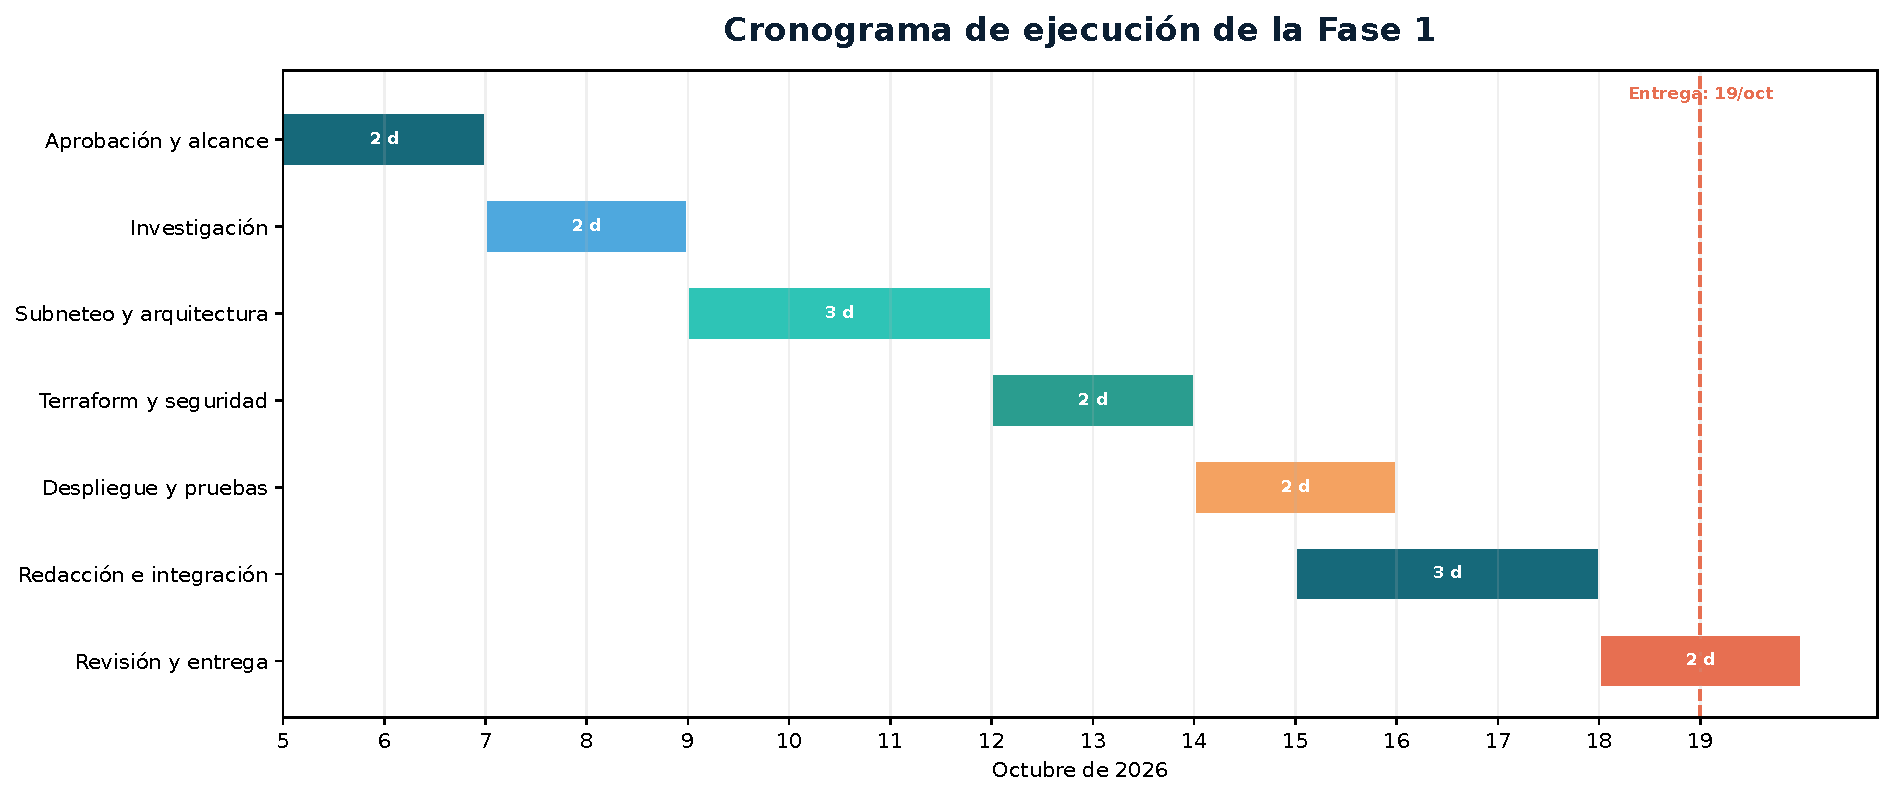
\includegraphics[width=\textwidth]{cronograma.pdf}
\caption{Cronograma de la Fase 1. Elaboración propia.}
\label{fig:gantt}
\end{figure}

\section{Responsabilidades}

\begin{table}[H]
\centering
\caption{Distribución propuesta de responsabilidades}
\begin{tabularx}{\textwidth}{p{4.5cm}Y Y}
\toprule
\textbf{Integrante} & \textbf{Responsabilidad principal} & \textbf{Revisión cruzada} \\
\midrule
Pablo Daniel Barillas Moreno & Coordinación, integración LaTeX, repositorio y compilación final. & Implementación y evidencias. \\
Andrés Rafael Chivalán & Cálculos de subneteo, arquitectura y consistencia de diagramas. & Revisión matemática y narrativa. \\
Roberto Emiliano Otoniel Camposeco Torres & Terraform, ejecución AWS, pruebas y destrucción. & Seguridad y anexos técnicos. \\
\bottomrule
\end{tabularx}
\end{table}

La asignación no elimina la responsabilidad conjunta. Toda modificación de direccionamiento debe ser revisada por otra persona; todo despliegue requiere confirmación del responsable de costos; y el PDF final debe ser leído por al menos dos integrantes.

\section{Hitos y puertas de calidad}

\begin{longtable}{p{2.2cm}p{4.1cm}p{7.1cm}}
\toprule
\textbf{Hito} & \textbf{Salida} & \textbf{Puerta de calidad} \\
\midrule
\endfirsthead
\toprule
\textbf{Hito} & \textbf{Salida} & \textbf{Puerta de calidad} \\
\midrule
\endhead
H1 & Alcance y supuestos & Cantidad de Visitas y composición del equipo visibles. \\
H2 & Selección de proveedor & Matriz ponderada, fuentes oficiales y decisión explicada. \\
H3 & Plan CIDR & Fórmulas, máscaras, reservas, rangos y script coinciden. \\
H4 & Código Terraform & Formato y validación sin errores; secretos excluidos. \\
H5 & Despliegue & Cuenta, región, costo y recursos identificados. \\
H6 & Pruebas & Ping real, prueba negativa y evidencia con fecha. \\
H7 & Cierre & Destrucción confirmada, PDF revisado y repositorio limpio. \\
\bottomrule
\end{longtable}

\section{Registro de riesgos}

\begin{longtable}{p{3.7cm}C{1.6cm}C{1.6cm}p{6.2cm}}
\toprule
\textbf{Riesgo} & \textbf{Prob.} & \textbf{Impacto} & \textbf{Respuesta} \\
\midrule
\endfirsthead
\toprule
\textbf{Riesgo} & \textbf{Prob.} & \textbf{Impacto} & \textbf{Respuesta} \\
\midrule
\endhead
Credenciales AWS ausentes & Alta & Alto & Configurar una identidad autorizada localmente; nunca copiar claves al informe o Git. \\
Permisos insuficientes & Media & Alto & Revisar errores por acción y ajustar sólo los permisos necesarios. \\
Cargos imprevistos & Media & Alto & Cómputo apagado por defecto, sin NAT, ventana corta y destrucción obligatoria. \\
CIDR incorrecto & Baja & Alto & Script de contención y no solapamiento antes de planificar. \\
SSH inaccesible & Media & Medio & Confirmar IP \code{/32}, reglas, llave y estado antes de probar. \\
ICMP bloqueado & Media & Medio & Verificar pertenencia al mismo SG y usar IP privada correcta. \\
Capturas ilegibles & Media & Medio & Recortar al recurso relevante y acompañar con pie explicativo. \\
PDF con desbordes & Baja & Medio & Renderizar todas las páginas e inspeccionar tablas y figuras. \\
Secreto en Git & Baja & Crítico & Revisar \code{git diff}, patrones de exclusión y escaneo textual antes del push. \\
\bottomrule
\end{longtable}

\section{Definición de terminado}

La fase se considera completa únicamente cuando: los requisitos tienen trazabilidad; los cálculos son reproducibles; Terraform valida; la infraestructura se despliega en una cuenta autorizada; el ping y el aislamiento producen evidencia; los recursos se destruyen; el PDF no presenta defectos; y el repositorio remoto contiene todos los entregables sin secretos. Si falta una condición, su estado se declara explícitamente.

\chapter{Control de costos y ciclo de vida}

\section{Principios adoptados}

El prototipo se diseña para existir durante minutos u horas, no durante todo el curso. El costo se controla con cinco decisiones: cómputo optativo, una sola dirección pública, ausencia de NAT Gateway, volúmenes mínimos y destrucción automatizada. Las subredes, tablas de rutas, grupos de seguridad e Internet Gateway no justifican por sí solos mantener instancias encendidas.

AWS publica un cargo horario por cada dirección IPv4 pública, tanto asociada como ociosa \cite{aws-vpc-pricing}. Por ello el bastión se crea sólo al habilitar la prueba y se destruye después de recopilar la salida. El diseño tampoco reserva una Elastic IP, evitando que una dirección permanezca en la cuenta tras apagar una instancia.

\section{Componentes potencialmente facturables}

\begin{table}[H]
\centering
\caption{Superficie de costo del prototipo}
\begin{tabularx}{\textwidth}{p{4.0cm}Y p{3.0cm}}
\toprule
\textbf{Componente} & \textbf{Control} & \textbf{Duración esperada} \\
\midrule
Tres instancias EC2 pequeñas & Activación explícita y destrucción tras pruebas. & Menos de 2 horas \\
Tres volúmenes GP3 de 8 GiB & Eliminación junto con las instancias. & Menos de 2 horas \\
Una IPv4 pública & Sólo en el bastión; no se reserva Elastic IP. & Menos de 2 horas \\
Transferencia de datos & Únicamente administración y paquetes de prueba. & Volumen mínimo \\
VPC y subredes & No requieren cómputo activo; se eliminan al final. & Ventana de prueba \\
\bottomrule
\end{tabularx}
\end{table}

No se fija un precio total en el informe porque las tarifas, impuestos, créditos, región y condiciones de la cuenta pueden cambiar. Antes del \code{apply}, el equipo debe consultar la página vigente de precios y el panel de facturación. Cualquier crédito académico se trata como beneficio eventual, no como garantía.

\section{Etiquetado}

Todos los recursos incorporan:

\begin{itemize}
  \item \code{Project=CC3067-Fase-1}
  \item \code{Group=Grupo-1}
  \item \code{Environment=academic-poc}
  \item \code{ManagedBy=Terraform}
  \item \code{DeleteAfter=2026-10-19}
\end{itemize}

Las etiquetas permiten filtrar componentes y detectar residuos. AWS recomienda rastrear recursos durante todo su ciclo de vida y usar etiquetas para identificar activos que pueden retirarse \cite{aws-track-resources}.

\section{Lista de cierre}

Después de \code{terraform destroy} se revisa:

\begin{enumerate}
  \item cero instancias con etiqueta del proyecto;
  \item cero volúmenes EBS residuales;
  \item cero direcciones públicas o Elastic IP del proyecto;
  \item cero interfaces de red huérfanas;
  \item Internet Gateway separado y eliminado;
  \item VPC y subredes eliminadas;
  \item estado local protegido y no agregado a Git;
  \item archivo \code{destroy.txt} con el resultado final.
\end{enumerate}

\begin{warningbox}[Regla de operación]
Detener una instancia no equivale a destruir todos sus recursos. La puerta de salida exige revisar volúmenes, IP, interfaces y gateways, no solamente el estado de EC2.
\end{warningbox}

\chapter{Conclusiones y recomendaciones}

\section{Conclusiones}

El diseño demuestra que las necesidades de RedNova GT caben holgadamente dentro de \code{10.10.0.0/24}. VLSM permite entregar capacidad distinta a cada departamento y reservar un cuarto del bloque para evolución. La selección no se basó únicamente en contar usuarios: también incorporó las cinco direcciones que AWS reserva por subred y el mínimo \code{/28} admitido por la plataforma.

Ventas ofrece el ejemplo más importante de juicio de ingeniería. Un \code{/27} satisface formalmente 25 usuarios, pero deja sólo dos direcciones asignables. Elegir \code{/26} aumenta el margen de operación y evita que una expansión pequeña obligue a migrar el segmento. TI requiere \code{/27}; Data Center utiliza \code{/28}; y Visitas recibe \code{/26} a partir del supuesto explícito de 30 clientes concurrentes.

La separación lógica se completa con enrutamiento y grupos de seguridad. Ventas, TI y Data Center carecen de ruta directa a Internet. El bastión temporal concentra la entrada administrativa y las instancias de prueba permanecen privadas. La prueba propuesta de ICMP usa la ruta local de la VPC y una regla auto-referenciada, por lo que valida conectividad interna sin exponer los hosts.

Terraform convierte la propuesta en un artefacto repetible, revisable y desmontable. La configuración pasó las pruebas locales de formato y validez, y el direccionamiento fue comprobado mediante un script independiente. No obstante, la estación de trabajo no dispone de credenciales AWS; por integridad académica, el informe identifica las pruebas cloud como pendientes y no inventa capturas ni resultados.

\section{Recomendaciones inmediatas}

\begin{enumerate}
  \item Configurar localmente una identidad AWS autorizada sin colocar secretos en el repositorio.
  \item Confirmar región, créditos, presupuesto y permisos antes de crear cómputo.
  \item Ejecutar el plan con \code{enable\_compute=false} y revisar primero la red.
  \item Generar una llave temporal y limitar \code{admin\_cidr} a la IPv4 real del operador.
  \item Activar cómputo, capturar las IP privadas y ejecutar las pruebas P-04 y P-05.
  \item Destruir inmediatamente y completar la prueba P-06.
  \item Incorporar capturas reales y recompilar el PDF antes de la entrega académica.
\end{enumerate}

\section{Evolución hacia producción}

Una fase posterior debería distribuir subredes en al menos dos zonas, incorporar acceso administrado sin bastión público, registros VPC Flow Logs, monitoreo, presupuestos, respaldos y una política IAM específica. También debe evaluar IPv6 y segmentar servicios por sensibilidad. Si se necesita salida desde subredes privadas, la elección entre NAT, endpoints o proxies debe basarse en flujos y costos medidos, no agregarse por defecto.

\section{Cierre}

La propuesta satisface el objetivo de diseño y deja una implementación técnicamente lista para una cuenta autorizada. Su principal fortaleza es la trazabilidad: cada requisito se conecta con un cálculo, un recurso, una prueba y una evidencia esperada. La condición restante no es de diseño ni de código, sino de acceso externo a AWS.

\appendix
\chapter{Inventario de archivos entregados}

\small
\begin{longtable}{p{5.3cm}p{8.0cm}}
\toprule
\textbf{Ruta} & \textbf{Propósito} \\
\midrule
\endfirsthead
\toprule
\textbf{Ruta} & \textbf{Propósito} \\
\midrule
\endhead
\path{docs/fase-1/main.tex} & Documento maestro LaTeX. \\
\path{docs/fase-1/preamble.tex} & Tipografía, colores, geometría y componentes visuales. \\
\path{docs/fase-1/sections/} & Capítulos modulares del informe. \\
\path{docs/fase-1/assets/diagrams/} & Diagramas PDF vectoriales y vistas PNG. \\
\path{docs/fase-1/assets/generated/} & Ilustración original de portada. \\
\path{docs/fase-1/assets/screenshots/} & Evidencias locales y de preparación incorporadas al informe. \\
\path{infra/terraform/} & VPC, subredes, rutas, seguridad, cómputo y salidas. \\
\path{scripts/generate-figures.py} & Generación reproducible de figuras con Matplotlib. \\
\path{scripts/validate-network.py} & Pruebas matemáticas del direccionamiento. \\
\path{scripts/test-connectivity.ps1} & Ping privado con salto SSH y registro de evidencia. \\
\path{scripts/build-report.ps1} & Generación de figuras, validación y compilación del PDF. \\
\path{evidence/} & Resultados verificables, salidas de Terraform y capturas genuinas de AWS. \\
\path{output/pdf/} & PDF final estable. \\
\href{https://github.com/DanielBarillasM/Proyecto-final_Grupo-1_Redes_Sec-10.git}{Repositorio GitHub del proyecto} & Código fuente, informe, scripts, evidencia permitida e historial de versiones. \\
\bottomrule
\end{longtable}
\normalsize

Las figuras se generaron con la interfaz orientada a objetos de Matplotlib y se exportaron como PDF vectorial y PNG de revisión. Esta metodología adopta prácticas de composición, accesibilidad y exportación documentadas en Scientific Agent Skills \cite{kassis2026skills}; el script queda incluido para que colores, etiquetas y datos puedan auditarse.

\chapter{Extractos de configuración}

\section{Definición de segmentos}

\begin{Verbatim}[fontsize=\footnotesize,frame=single]
subnets = {
  visitas        = { cidr = "10.10.0.0/26",   public = true  }
  ventas         = { cidr = "10.10.0.64/26",  public = false }
  ti             = { cidr = "10.10.0.128/27", public = false }
  datacenter     = { cidr = "10.10.0.160/28", public = false }
  administracion = { cidr = "10.10.0.176/28", public = true  }
}
\end{Verbatim}

\section{Regla ICMP de Ventas}

\begin{Verbatim}[fontsize=\footnotesize,frame=single]
ingress {
  description = "ICMP entre miembros del mismo grupo"
  from_port   = -1
  to_port     = -1
  protocol    = "icmp"
  self        = true
}
\end{Verbatim}

\section{Salidas relevantes}

\begin{Verbatim}[fontsize=\footnotesize,frame=single]
output "bastion_public_ip" {
  value = try(aws_instance.bastion[0].public_ip, null)
}

output "ventas_private_ips" {
  value = aws_instance.ventas[*].private_ip
}
\end{Verbatim}

\chapter{Procedimiento operativo abreviado}

\begin{enumerate}
  \item Autenticarse en AWS por un mecanismo local autorizado.
  \item Consultar identidad y región sin registrar secretos.
  \item Generar llave SSH temporal.
  \item Copiar y completar \code{terraform.tfvars.example}.
  \item Ejecutar \code{terraform init}, \code{fmt}, \code{validate} y \code{plan}.
  \item Revisar el plan con otro integrante.
  \item Aplicar y esperar estado saludable de las instancias.
  \item Ejecutar \code{scripts/test-connectivity.ps1} con las salidas obtenidas.
  \item Capturar VPC, subredes, rutas, reglas, instancias y resultados.
  \item Ejecutar \code{terraform destroy}.
  \item Auditar la ausencia de recursos etiquetados.
  \item Recompilar, inspeccionar el PDF y publicar el repositorio.
\end{enumerate}

\begin{thebibliography}{99}
\addcontentsline{toc}{chapter}{Referencias}

\bibitem{aws-subnet-sizing}
Amazon Web Services, ``Subnet CIDR blocks'', \emph{Amazon VPC User Guide}. Disponible en: \url{https://docs.aws.amazon.com/vpc/latest/userguide/subnet-sizing.html}. Consultado el 5 de octubre de 2026.

\bibitem{aws-configure-subnets}
Amazon Web Services, ``Subnets for your VPC'', \emph{Amazon VPC User Guide}. Disponible en: \url{https://docs.aws.amazon.com/vpc/latest/userguide/configure-subnets.html}. Consultado el 5 de octubre de 2026.

\bibitem{aws-route-tables}
Amazon Web Services, ``Subnet route tables'', \emph{Amazon VPC User Guide}. Disponible en: \url{https://docs.aws.amazon.com/vpc/latest/userguide/subnet-route-tables.html}. Consultado el 5 de octubre de 2026.

\bibitem{aws-internet-gateway}
Amazon Web Services, ``Enable internet access for a VPC using an internet gateway'', \emph{Amazon VPC User Guide}. Disponible en: \url{https://docs.aws.amazon.com/vpc/latest/userguide/VPC_Internet_Gateway.html}. Consultado el 5 de octubre de 2026.

\bibitem{aws-vpc-pricing}
Amazon Web Services, ``Amazon VPC pricing''. Disponible en: \url{https://aws.amazon.com/vpc/pricing/}. Consultado el 5 de octubre de 2026.

\bibitem{aws-decommission}
Amazon Web Services, ``Decommission resources'', \emph{AWS Well-Architected Framework: Cost Optimization Pillar}. Disponible en: \url{https://docs.aws.amazon.com/wellarchitected/latest/cost-optimization-pillar/decommission-resources.html}. Consultado el 5 de octubre de 2026.

\bibitem{aws-track-resources}
Amazon Web Services, ``COST04-BP01 Track resources over their lifetime'', \emph{AWS Well-Architected Framework}. Disponible en: \url{https://docs.aws.amazon.com/wellarchitected/latest/framework/cost_decomissioning_resources_track.html}. Consultado el 5 de octubre de 2026.

\bibitem{terraform-install}
HashiCorp, ``Install Terraform'', \emph{HashiCorp Developer}. Disponible en: \url{https://developer.hashicorp.com/terraform/tutorials/aws-get-started/install-cli}. Consultado el 5 de octubre de 2026.

\bibitem{kassis2026skills}
T. Kassis, V. Agarwal, Y. He, D. Patel y A. M. Brueckner, ``Scientific Agent Skills: A Library of Procedural Knowledge for Research Agents'', \emph{arXiv:2609.00065}, 2026. doi: \url{https://doi.org/10.48550/arXiv.2609.00065}.

\end{thebibliography}


\end{document}
